% This project is part of the Continuous-Function Estimator project
% Copyright 2019 the authors.

% to-do
% -----

% style notes
% -----------
% - line break at sentence breaks

%\documentclass[twocolumn]{aastex62}
%\documentclass[12 pt]{article}
\documentclass[modern]{aastex62}

\usepackage[sort&compress]{natbib}
\usepackage{graphicx}
\graphicspath{ {./images/} }
\usepackage{xspace}
\usepackage{xcolor}
\usepackage{bm}
\usepackage{mathtools}
\parindent=19pt

% aastex parameters
%%\hypersetup{linkcolor=red,citecolor=green,filecolor=cyan,urlcolor=magenta}
\received{XXX}
%\revised{not yet}
\accepted{YYY}
%\submitjournal{ApJ}
\shorttitle{a continuous correlation function estimator}
\shortauthors{storey-fisher and hogg}

% language
\newcommand{\cf}{2pcf\xspace} %2pF? 2PCF? %TODO: fix spacing after
% to capitalize or not to capitalize? leaning no
\newcommand{\Est}{The Continuous-Function Estimator\xspace}
\newcommand{\est}{the Continuous-Function Estimator\xspace}
\newcommand{\documentname}{\textsl{Article}\xspace}
\newcommand{\LS}{LS\xspace}
\newcommand{\foreign}[1]{\textsl{#1}}
\newcommand{\etc}{\foreign{etc}}
\newcommand{\eqt}[1]{equation~(\ref{#1})}

% math
\newcommand{\inv}{^{-1}}
\newcommand{\invp}{^{'-1}}
\newcommand{\T}{^{\mathsf{T}}}
\newcommand{\Tp}{^{'\mathsf{T}}}
\newcommand{\hmpc}{$h^{-1}\,$Mpc}
\newcommand{\dd}{\mathrm{d}}
\newcommand{\bld}[1]{\bm{#1}} %\mathbf gives very different look!
\newcommand{\vv}[1]{\bld{v}_\mathrm{#1}}
\newcommand{\TT}[1]{\bld{T}_\mathrm{#1}}
\newcommand{\ff}{\bld{f}}
\newcommand{\NN}[1]{N_\mathrm{#1}}
\newcommand{\GG}[1]{\mathsf{G}_{#1}}

% comments
\newcommand{\KSF}[1]{\textcolor{teal}{KSF says: #1}}
%\newcommand{\KSF}[1]{\textcolor{teal}{}} #to see doc w/o comments
\newcommand{\hogg}[1]{\textcolor{red}{Hogg says: #1}}

% margins
%\addtolength{\topmargin}{-0.75in}
%\addtolength{\textheight}{1.50in}

% affiliations
\newcommand{\ccpp}{\affiliation{%
    Center for Cosmology and Particle Physics,
    Department of Physics,
    New York University}}
\newcommand{\flatiron}{\affiliation{%
    Flatiron Institute, Simons Foundation}}
\newcommand{\cds}{\affiliation{%
    Center for Data Science,
    New York University}}
\newcommand{\mpia}{\affiliation{%
    Max-Planck-Institut f\"{u}r Astronomie, Heidelberg}}


\begin{document}\sloppy\sloppypar\raggedbottom\frenchspacing

\title{\textbf{Two-point statistics without bins: A continuous-function generalization of the correlation function estimator for large-scale structure}}

\author[0000-0001-8764-7103]{Kate Storey-Fisher}
\ccpp

\author[0000-0003-2866-9403]{David W. Hogg}
\ccpp
\cds
\mpia
\flatiron

\begin{abstract}\noindent
% Context / Aims
The two-point correlation function (\cf) is the most important statistic in structure formation, used to measure the clustering of density field tracers (e.g., galaxies).
Current estimators of the 2pcf, including the standard Landy--Szalay (\LS) estimator, evaluate the \cf in hard-edged bins of separation between objects; this is inappropriate for the science context and results in a loss of information and a poor trade-off between bias and variance.
%Methods
We present a new estimator for the \cf, \emph{\est}, which generalizes \LS to a continuous representation and obviates binning in separation or any other pair property. 
Our estimator replaces the binned pair counts with a linear superposition of basis functions; it outputs the best-fit linear combination of basis functions to describe the \cf. 
It is closely related to the estimator used in linear least-squares fitting. 
The choice of basis can take into account the expected form of the \cf, as well as its dependence on properties other than pair separation (e.g., stellar mass or sky position).
%Results
We show that \est with a choice of cubic-spline basis functions better represents the smoothness and shape of the \cf compared to \LS.
We further demonstrate that the estimator can be used to directly estimate the Baryon Acoustic Oscillation scale, using a small number of physically motivated basis functions.
Critically, the reduction in the number of basis functions leads to a reduction in the number of mock catalogs required for covariance estimation; this is currently the limiting step in many \cf measurements.
We discuss applications and limitations of \est for present and future studies of large-scale structure, including determining the dependence of clustering on galaxy properties and investigating potential inhomogeneities or anisotropies in clustering.
\end{abstract}

%TODO: should have 6 keywords 
%via Unified Astronomy Thesauras (UAT), http://astrothesaurus.org/concept-select/
\keywords{Astrostatistics techniques (1886), Baryon acoustic oscillations (138), Cosmology (343), Two-point correlation function (1951), Large-scale structure of the universe (902), Redshift surveys (1378)}

\section{Introduction}

The large-scale structure (LSS) of the Universe is critical to our understanding of fundamental cosmology. 
It encodes information about the physics of the early Universe and the subsequent expansion history. \KSF{cite something here - zeldovich or something. maybe 2, one for early u and one for expansion history.}
In particular, LSS measures the Baryon Acoustic Oscillation (BAO) scale \citep{Eisenstein2005}, which results from density fluctuations in the baryon--photon fluid.
The distance traveled by these density waves before recombination imprints a feature on the statistical description of the LSS, which can be used to determine the characteristic BAO length scale \citep{PeeblesYu1970, EisensteinHu1998}.
The LSS also contains the signature of redshift-space distortions caused by the peculiar velocities of galaxies, which are used to measure the growth rate of structure \citep{Kaiser1987}.
Additionally, the LSS can be used to constrain galaxy formation in conjunction with models of galaxy bias (e.g., \citealt{Hamilton1988}, \citealt{Budavari2003}, \citealt{Li2006}, \citealt{Abbas2006}, \citealt{Zehavi2011}, \citealt{Skibba2014}, \citealt{Durkalec2018}). \KSF{do i not need all these citations here? do i need more elsewhere in the intro?}
With current observations, the LSS is well-described by a cold dark matter model with a cosmological constant, the standard $\Lambda$CDM model. \KSF{cite construction of lcdm model, and another for fact that good fit to obs}
Upcoming galaxy surveys will observe larger volumes with improved measurements, allowing us to test $\Lambda$CDM to even higher precision. \KSF{cite desi, euclid, rubin}

The most important statistic for characterizing the LSS is the two-point correlation function (\cf).
It measures the excess frequency at which any two galaxies are separated by a given distance, compared to a uniform distribution; effectively, it characterizes the strength of clustering at a given spatial scale.
The \cf is the primary tool for extracting cosmological information from galaxy redshift surveys.
Such correlation function analyses include \cite{Hawkins2003} for the 2dF Galaxy Redshift Survey (2dFGRS, \citealt{Colless2001}), \cite{Alam2016} for the Baryon Oscillation Spectroscopic Survey (BOSS, \citealt{Dawson2013}) DR12 analysis, and \cite{Elvin-Poole2017} for the Dark Energey Survey (DES, \citealt{DES2005}).

Estimators of the \cf have been studied extensively (e.g., \citealt{PeeblesHauser1974}; \citealt{DavisPeebles1983}; \citealt{Hamilton1993}).
Traditionally, the \cf is estimated in bins of radial separation.
This binning introduces inherent limitations.
First, the choice of bins requires a trade-off between bias and variance: fewer bins may bias the result, while more bins increases the variance of measurement.
Finite-width bins also result in a loss of information about the property in which one is binning.
As we work towards extreme precision in large-scale structure, maximizing the information we extract with our analyses will become increasingly important.
Additionally, the error on the inverse covariance matrix estimate depends on the number of bins, with a larger number of bins resulting in a larger error that propogates to the estimated parameters \citep{Hartlap2007, Percival2014}.
This can be balanced by using a large number of mock galaxy catalogs, but these can be exceedingly expensive to generate.
This is currently the limiting step in LSS analyses, with on the order of 1000 mock catalogs tailored to the survey needed to achieve the desired precision on the parameters.
The requirements on the covariance matrix will get even more stringent as survey size increases and we push towards higher precision; the connection of this liming step with bin choice merits scrutiny of binning in \cf analyses.

More generally, binning adds arbitrary boundaries between continuous data; results should not depend on bin choice, yet they sometimes do.
\cite{Lanzuisi2017} noted that the choice of binning axis impacts the detected correlation between the luminosity of active galactic nuclei and their host galaxies; \cite{Grimmett2020} devised a method to investigate this correlation in a continuous manner using a hierarchical Bayesian model, eliminating the need for binning.
\cite{Bailoni2016} explored the dependence of clustering analyses on the number of redshift bins, finding a non-negligible difference in cosmological parameter uncertainties.
The implications for BAO analyses were explored by \cite{Percival2014}, who found that the effects of bin width are small but non-negligible; they showed that there is an optimal bin width given the analysis method that trades off statistical uncertainty against bias in the derived BAO peak location.
From this literature, it is clear that, when analyzing smooth quantities such as LSS statistics, binning is sinning.

One of the difficulties in performing a two-point estimate is that nontrivial survey boundaries would bias a direct summation of pair counts.
To account for the boundaries as well as regions corrupted by issues such as bright foreground stars, typically a large set of random points are Poisson-distributed within the acceptable survey window.
The pairwise correlations of these unclustered points are used to normalize out the survey window.
The current standard estimator, proposed by \cite{LandySzalay1993} (hereafter \LS), takes this approach.
It involves a summation of the data--data pairs $DD$ in each separation bin, normalized by random--random pairs $RR$ as well as the data--random pairs $DR$ to improve the bias properties of the estimator.
The \LS estimator of the correlation function $\hat{\xi}_k$ for the $k^\mathrm{th}$ bin in separation $r$ is defined as
\begin{equation} \label{eq:lsintro}
\hat{\xi}_k = \frac{DD_k - 2DR_k + RR_k}{RR_k} ~.
\end{equation}
Compared with other estimators based on simple combinations of $DD$, $DR$ and $RR$, \LS has been shown to have the lowest bias and variance \citep{Kerscher2000}.
Estimators of the \cf must also take into account the imperfect nature of the survey, including systematic effects, the target completeness, and fiber collisions.
To account for these, each galaxy pair is sometimes assigned a weight, and pair counts are replaced by the sum of pair weights.

Variations on traditional \cf estimation have been proposed in recent years.
\cite{Demina2016} replaced the $DR$ and $RR$ terms with an integral over the probability map, reducing computation time and increasing precision.
An estimator proposed by \cite{VargasMagana2013} iterates over sets of mock catalogs to find an optimal linear combination of data and random pair counts, reducing the bias and variance.
An alternative estimator, the marked correlation function (e.g., \citealt{WhitePadmanabhan2009}), avoids the use of a random catalog altogether: it considers the ratio between the \cf and a weighted correlation function in which weights are assigned based on galaxy properties, such as the local density.
These estimators have all taken probabilistic approaches; others have taken a likelihood approach.
\cite{BaxterRozo2013} introduced a maximum likelihood estimator for the \cf, which achieves lower variance compared to the \LS estimator, enabling finer binning and requiring a smaller random catalog for the same precision.
% TODO: kernel methods to cite and destroy here?
% minimal in intro: after lit review ("variations" paragraph) - in some ways what we're doing bears some resemblance to mcf, because we're weighting the pairs by functions, and kernel estimates bc we're projecting the pairs onto basis functions; we will discuss below that our method is distinct from both of these approaches. think of this careful address as talking to referree or referree-like reader

These estimators present improvements to \LS, but they are still limited to estimates in separation bins.
Some require additional computational costs or layers of complexity, so the standard formulation of \LS continues to be the default estimator used in most analyses.

In this \documentname, we present a new estimator for the correlation function, \est, which generalizes the \LS estimator to produce a continuous estimation of the \cf. 
\Est projects the galaxy pairs onto a set of continuous basis functions and directly computes the best-fit linear combination of these functions.
The basis representation can depend on the pair separation as well as other desired properties, and can also utilize the known form of the \cf.
For tophat basis functions, the estimator exactly reduces to the \LS estimator. 
\Est removes the need for binning and produces a more representative estimate of the \cf with fewer basis functions, reducing requirements on mock catalogs for covariance matrix computation.
It is particularly well-suited to the analysis of LSS features such as the BAO peak; we find that we can accurately locate the peak with fewer components compared to standard analyses.

This \documentname is organized as follows. 
In Section~\ref{sec:motiv}, we motivate our estimator and explain its formulation.
We demonstrate its application on a simulated data set, including a toy BAO analysis, in Section~\ref{sec:experiments}.
We discuss the implications and other possible applications in Section~\ref{sec:discuss}. 

\section{Motivation and Formulation} 
\label{sec:motiv}

In this \documentname, we use the following notation.
We write vectors in bold and lowercase, e.g. $\vv{}$; tensors in bold and uppercase, e.g. $\TT{}$; and unstructured data blobs in sans serif, e.g. $\GG{}$.
A hat above a symbol, e.g. $\bld{\hat{\xi}}$, indicates an estimate of the value.

\subsection{Standard Two-Point Correlation Function Estimation}

The standard approach to estimating the two-point correlation function involves counting pairs of tracers within a survey volume as a function of separation scale.
Let's assume we have a data catalog with $N_D$ objects within a sky volume.
We also require a random catalog with $N_R$ objects distributed uniformly throughout the same volume.
We can define a set of separation bins which we will use to estimate the \cf at various scales.
We are then ready to sum in each bin the relevant pairs of objects within and across our catalogs.
In standard notation, these pair counts are written as $DD$, $DR$, and $RR$, as in \eqt{eq:lsintro}.
To clarify that these are in fact vectors, with length $K$ where $K$ is the number of bins, we use the symbol $\vv{}$; then, for example, the data--data pair counts $DD$ become $\vv{DD}$.
We can then write the \LS estimator as 
\begin{equation} \label{eq:ls}
    \bld{\hat{\xi}} = \frac{\vv{DD} - 2\,\vv{DR} + \vv{RR}}{\vv{RR}} ~.
\end{equation}
The components of the pair-count vectors are defined explicitly as
\begin{eqnarray}\displaystyle
    \label{eq:ls1}
    % \adjustlimits aligns the subscripts with and without primes, which are diff heights
    \left[ \vv{DD} \right]_k &\equiv& \frac{2}{\NN{D}\,(\NN{D}-1)} \adjustlimits \sum_{n} \sum_{n' < n} i(g_k < |\bld{r}_n - \bld{r}_{n'}| < h_k) \\ 
    \left[ \vv{DR} \right]_k &\equiv& \frac{1}{\NN{D}\,\NN{R}} \sum_{n} \sum_{m} i(g_k < |\bld{r}_n - \bld{r}_m| < h_k) \\
    \label{eq:ls3}
    \left[ \vv{RR} \right]_k &\equiv& \frac{2}{\NN{R}\,(\NN{R}-1)} \adjustlimits\sum_{m} \sum_{m'<m} i(g_k < |\bld{r}_m - \bld{r}_{m'}| < h_k) ~,
\end{eqnarray}
where $\left[ \vv{} \right]_k$ is the pair counts in bin $k$ (which has bin edges $g_k$ and $h_k$), $i$ is an indicator function that returns $1$ if the the condition is true and otherwise returns $0$, $\bld{r}$ is the tracer position, the $n$ and $n'$ indices index data positions, and the $m$ and $m'$ indices index random catalog positions.
The sums are over unique pairs, and for auto-correlations they exclude self-pairs; the normalization prefactors then account for the total number of possible pairs, explaining the difference between the auto- and cross-correlation factors.
The tracer position can be in real or redshift space, or broken down into the transverse and line-of-sight directions in the anisotropic correlation function; in this \documentname we consider the isotropic real-space \cf for simplicity, but the estimators detailed here apply equally well to these alternative configurations.
The estimator is also easily applicable to cross-correlations of two data sets.
 
The \LS estimator is known to be optimal (i.e. it is unbiased and has minimum variance) under a particular set of conditions: in the limit of unclustered data, for a data volume much larger than the scales of interest, and an infinitely large random catalog. 
In practice the latter two limits are sufficiently satisfied, but the data we are interested in are clustered.
\cite{VargasMagana2013} show that for clustered data, the \LS estimator has lower variance than other estimators, but does not reach the Poisson noise limit.
When applied to clustered data, \LS does show a bias on very large scales ($>$130 \hmpc), but the bias is significantly smaller than that of most other estimators (\citealt{Kerscher1999}, \citealt{VargasMagana2013}).
\LS is also less sensitive to the number of random points than other estimators \citep{Kerscher2000}.
While \LS has been sufficient for past analyses, its persisting bias and suboptimal variance under imperfect conditions mean that improvement is possible, and will be necessary for realistic large-scale structure measurements on modern datasets.

\subsection{Least Squares Fitting}

Clustering estimation is closely related to least-squares fitting.
We are essentially trying to find the best representation of spatial data in the space of two-point radial separation.
Recall that the linear least-squares fit to a set of data is
\begin{equation}
    \label{eq:leastsq}
    \bld{x} = [\bld{A}\T\,\bld{C}\inv\,\bld{A}]\inv \, [\bld{A}\T\,\bld{C}\inv\,\bld{y}] ~,
\end{equation}
where $\bld{x}$ is the vector of best-fit parameters, $\bld{A}$ is a design matrix containing functions of fitting features, $\bld{C}$ is the covariance matrix, and $\bld{y}$ is a column vector of $\bld{y}$ data to be fit.
The second bracketed factor $[\bld{A}\T\,\bld{C}\inv\,\bld{y}]$ projects the data onto the features (as in a matched filter). 
The first bracketed factor $[\bld{A}\T\,\bld{C}\inv\,\bld{A}]\inv$ rescales the projected features into the space of the parameters.

Standard two-point correlation function estimators are effectively performing such a projection: each bin is the projection of the data pair counts onto the radial separation annulus, and the random-random term rescales this feature.
The analogy is clear in the so-called natural estimator of the \cf, $\bld{\hat{\xi}} = \vv{DD}/\vv{RR} - 1$ (e.g., \citealt{Kerscher2000}), with $\vv{DD}$ aligning with the second bracketed factor and $\vv{RR}$ aligning with the first (the division can be written as an inverse factor).
\Est was inspired by this connection with least-squares fitting; we detail its formulation in the following section.


\subsection{\Est}
\label{sec:est}

We generalize the \LS estimator defined above in equations~(\ref{eq:ls1}--\ref{eq:ls3}) by analogy with least-squares fitting.
We generalize the indicator function $i$ to any function $\ff$, which returns a vector of length $K$ where $K$ is the number of basis functions.
We further generalize the arguments of the function to any properties of the galaxy pair, rather than just the separation between pairs; we call $\GG{ij}$ the data payload for the pair of galaxies $i$ and $j$.
This gives us, instead of pair counts, a vector $\vv{}$ of \textit{projections} of the basis functions.
These projection vectors are defined as
\begin{eqnarray}\displaystyle
    \vv{DD} &\equiv& \frac{2}{\NN{D}\,(\NN{D}-1)} \adjustlimits \sum_{n} \sum_{n'<n} \ff(\GG{n n'}) \\
    \vv{DR} &\equiv& \frac{1}{\NN{D}\,\NN{R}} \sum_{n} \sum_{m} \ff(\GG{n m}) \\
    \vv{RR} &\equiv& \frac{2}{\NN{R}\,(\NN{R}-1)} \adjustlimits \sum_{m} \sum_{m'<m} \ff(\GG{m m'}) \\
    \TT{RR} &\equiv& \frac{2}{\NN{R}\,(\NN{R}-1)} \adjustlimits \sum_{m} \sum_{m'<m} \ff(\GG{m m'}) \cdot \ff\T(\GG{m}, \GG{m'}) \label{eq:qq_proj} ~,
\end{eqnarray}
where the prefactors are as explained for the standard \LS estimator.

We can now define \est as
\begin{equation}
    \label{eq:xi_proj}
    \hat{\xi}(\GG{ll'}) \equiv \bld{a}\T \cdot \ff(\GG{ll'}) ~,
\end{equation}
where $\bld{a}$ is a $K$-vector of the computed \emph{amplitudes} of the basis functions
\begin{equation}
    \label{eq:amplitude}
    \bld{a} \equiv \TT{RR}\inv \cdot (\vv{DD} - 2\,\vv{DR} + \vv{RR})
\end{equation}
and $\GG{ll'}$ contains the data values at which to evaluate $\bld{\hat{\xi}}$.
Note that we do not bold $\hat{\xi}$ in $\hat{\xi}(\GG{ll'})$ as this indicates the evaluation of the \cf at a particular point in parameter space, which outputs a scalar, while in the form $\bld{\hat{\xi}}$ we are representing the full vector output of the estimator.

The choices in this formulation are explained by analogy with least-squares fitting.
In the amplitudes $\bld{a}$, the linear combination of vectors $(\vv{DD} - 2\,\vv{DR} + \vv{RR})$ projects the pair information onto the features; the $\TT{RR}\inv$ factor rescales these projected features into the space of the parameters of $\bld{\hat{\xi}}$.
This then explains the formulation of the $\TT{RR}$ factor: we require an invertible matrix to perform the rescaling, and in the case of the \cf the rescaling of the data is performed by the autocorrelation of the random catalog.
The exact formulation of this factor as the sum of outer products of the basis function vectors and their transposes is motivated by the desire that the estimator be invariant under affine transformations, such as a rescaling of the basis functions or a rotation in the basis space (see Appendix~\ref{sec:affine}).

We emphasize that $\GG{ll'}$ in \eqt{eq:xi_proj} does not represent a real pair of galaxies, but instead allows us to evaluate the \cf at any set of parameters.
In the standard case (see \eqt{eq:ff_separation} below), $\GG{ll'}$ would effectively be the data for imaginary pair of galaxies $l$ and $l'$ that have a separation $r$ at which we want to evaluate $\bld{\hat{\xi}}$, and we would compute $\bld{\hat{\xi}}$ for such a pair at every separation in which we are interested.
With our general formulation, we could choose basis functions that depend on other galaxy properties (see Section~\ref{sec:applications}); then, we would also choose each $\GG{ll'}$ pair to have values of these properties at which we want to evaluate $\bld{\hat{\xi}}$.
In the experiments in this \documentname, however, we will only take into account the separation between pairs, so we will write $\hat{\xi}(r)$.

\Est can be straightforwardly generalized to cross-correlations between two datasets.
In this case, we consider datasets $D_1$ and $D_2$, and associated random catalogs $R_1$ and $R_2$. 
We then have cross-correlations rather than auto-correlations for the data-data and random-random terms, and two different data-random terms, crossing each dataset with the opposite random catalog. 
The data-data term becomes 
\begin{equation}
    \vv{D_1 D_2} \equiv \frac{1}{\NN{D_1}\,\NN{D_2}} \sum_{n_1} \sum_{n_2} \ff(\GG{n_1 n_2}) ~,
\end{equation}
where $n_1$ and $n_2$ index the data points in each catalog, and the normalization factor is now simply the product of catalog sizes as we are no longer concerned with double-counting.
The other terms ($\vv{D_1 R_2}$, $\vv{D_2 R_1}$, $\vv{R_1 R_2}$, $\TT{R_1 R_2}$) generalize as one would expect.
The amplitudes then become
\begin{equation}\displaystyle
    \bld{a} \equiv \TT{R_1 R_2}\inv \cdot (\vv{D_1 D_2} - \vv{D_1 R_2} - \vv{D_2 R_1} + \vv{R_1 R_2})
 \end{equation}
and we use this to compute the estimator as in \eqt{eq:xi_proj}.

If we consider only the pair separation, and make a proper choice of $\ff$, \est reduces to the \LS estimator.
Explicitly, from our full galaxy pair data $\GG{n n'}$, we can use only their separation,  $|\bld{r}_n - \bld{r}_{n'}|$.
We can then define a set of $K$ basis functions $\ff$ as
\begin{equation}
    \label{eq:ff_separation}
    \ff_k(\GG{n n'}) =  i(g_k < |\bld{r}_n - \bld{r}_{n'}| < h_k) ~.
\end{equation}
This is the common tophat (or rectangular) function; the index $k$ denotes a particular bin in separation, and here also indexes the basis functions, as each top-hat is a separate basis function.
In this case the $\vv{DD}$, $\vv{DR}$ and $\vv{RR}$ projection vectors simply become binned pair counts, with bin edges $g_k$ and $h_k$ as before.
The $\TT{RR}$ tensor becomes diagonal, with its diagonal elements equal to the elements of the $\vv{RR}$ vector.
Then the evaluation of the amplitudes $\bld{a}$ and the correlation function estimate $\bld{\hat{\xi}}$ results in the equivalent of the \LS estimator--just displayed in a continuous form.

We call this generalized \cf estimator \est.
It replaces the binned pair counts of \LS with any set of basis functions; the linear superposition of these basis functions is our estimate of the \cf.
Essentially, \est outputs the best-fit linear combination of basis functions to describe the \cf.
In this sense, it is deeply related to the linear least-squares fitting described above.
With our formulation, we no longer need to first bin our data and then fit a function; rather, the estimator directly projects the data (the pair counts) onto the desired function.
This function can be nearly anything; the only limitation is it must be able to be written as a linear combination of basis functions.

With this generalized two-point estimator, the basis functions need not have hard edges like the tophat function.
They can instead be smooth functions of the pair separation, or chosen to suit the science use case.
Further, the bases can make use of other information about the tracers or the survey; they are extremely general.
The estimator also has the property that it is invariant under affine transformations, as it should be so that the result does not depend on e.g. the magnitude of the bases; we show this in Appendix~\ref{sec:affine}.

We can also write down the form of \est when we are working with a periodic box and don't need to worry about the survey window.
In this case, we can analytically compute the $\vv{RR}$ term, as well as the $\TT{RR}$ term, and use the natural form of the \cf estimator.
The derivation and formulation of these terms are shown in Appendix~\ref{sec:analytic}.

We implement this estimator based on the correlation function package \texttt{Corrfunc} by \cite{Sinha2019}.
\texttt{Corrfunc} is the state-of-the-art package for computing correlation functions and other clustering statistics; it is extremely fast and user-friendly, and is used in many published analyses.
It is also modular and open-source, making it a natural choice as a base for our implementation.
Our implementation of \est is also open-source and available at \texttt{github.com/kstoreyf/Corrfunc}.
Implementation details are discussed in Section~\ref{sec:comp}.


\section{Experiments and Results}
\label{sec:experiments}

\subsection{Lognormal Mock Catalogs}

We demonstrate the application of \est on a set of artifical data.
We generate lognormal mock catalogs \citep{ColesJones1991} using the \texttt{lognormal\_galaxies} code by \citep{Agrawal2017}.
We use an input power spectrum with the Planck cosmology, the same parameters used for the MultiDark--PATCHY simulations \citep{Kitaura2016} made for the Baryon Oscillation Spectroscopic Survey (BOSS, \citealt{Dawson2013}.
This assumes a cold dark matter model with $\Omega_m = 0.307115$, $\Omega_b = 0.048206$, $\sigma_8 = 0.8288$, $n_s = 0.9611$, and $h = 0.6777$.
Our fiducial test set is 1000 realizations of periodic cubes with size (750 \hmpc)$^3$ and a galaxy number density of $2 \times 10^{-4}$ $h^{3}\,$Mpc$^{-3}$.
We choose to perform these tests on periodic boxes so that we may compute the random--random term analytically (see Appendix~\ref{sec:analytic}), significantly cutting down on computation time.
The results will hold for catalogs with realistic survey windows and random--random terms computed directly with \est.

\subsection{Comparison of Standard Tophat Basis Functions}

We first estimate the correlation function of our mocks using the the standard estimator.
We choose 15 separation ($r$) bins in the range $36 < r < 156$ \hmpc, each with a width of 8 \hmpc; this was found to be the optimal bin width by \cite{Percival2014}, and is standard for two-point analyses.
We apply the estimator to each of our 1000 mock catalogs.
The mean of these estimated correlation functions is shown in Figure~\ref{fig:tophat}; the error bars show the standard deviation of the 1000 mocks in each bin.
We also show the true input correlation function, and the bottom panel shows the absolute error between the estimated and true correlation functions.

There remains an ambiguity in the $r$-value at which to plot the result of the standard estimator. 
The volume-weighted average is often used, or a weighted average depending on the pairs in the bin; this choice propagates to differences in comparing the estimate to models (though at the precision of current surveys these differences are not significant).
Here we plot the standard estimator with the volume-weighted average.

We demonstrate \est with a tophat basis function.
We choose tophat functions with the same locations and widths as the bins used for the standard estimator; these are shown in the top panel of Figure~\ref{fig:tophat}. 
As this estimator computes the \cf in a continuous form, we plot the result as a continuous function at every $r$-value.
In practice, this means choosing a fine grid of $r$-values at which to evaluate $\hat{\xi}(r)$; here we choose 1000 $r$-values across the separation range.
This results in a step function form for the correlation function.
The values of the correlation function at each step exactly align with the result of the standard estimator.
In fact, we emphasize that this step function is exactly what the standard estimator is estimating; we have just made explicit the fact that the each estimate applies to the entire bin.
When we look at the error with respect to the truth (bottom panel), the error blows up at the edges of each bin, where the continuous estimate deviates most significantly from the truth.
This demonstrates one way in which the standard tophat estimator is not a good representation of the true \cf.

\begin{figure}[t]
\centering
    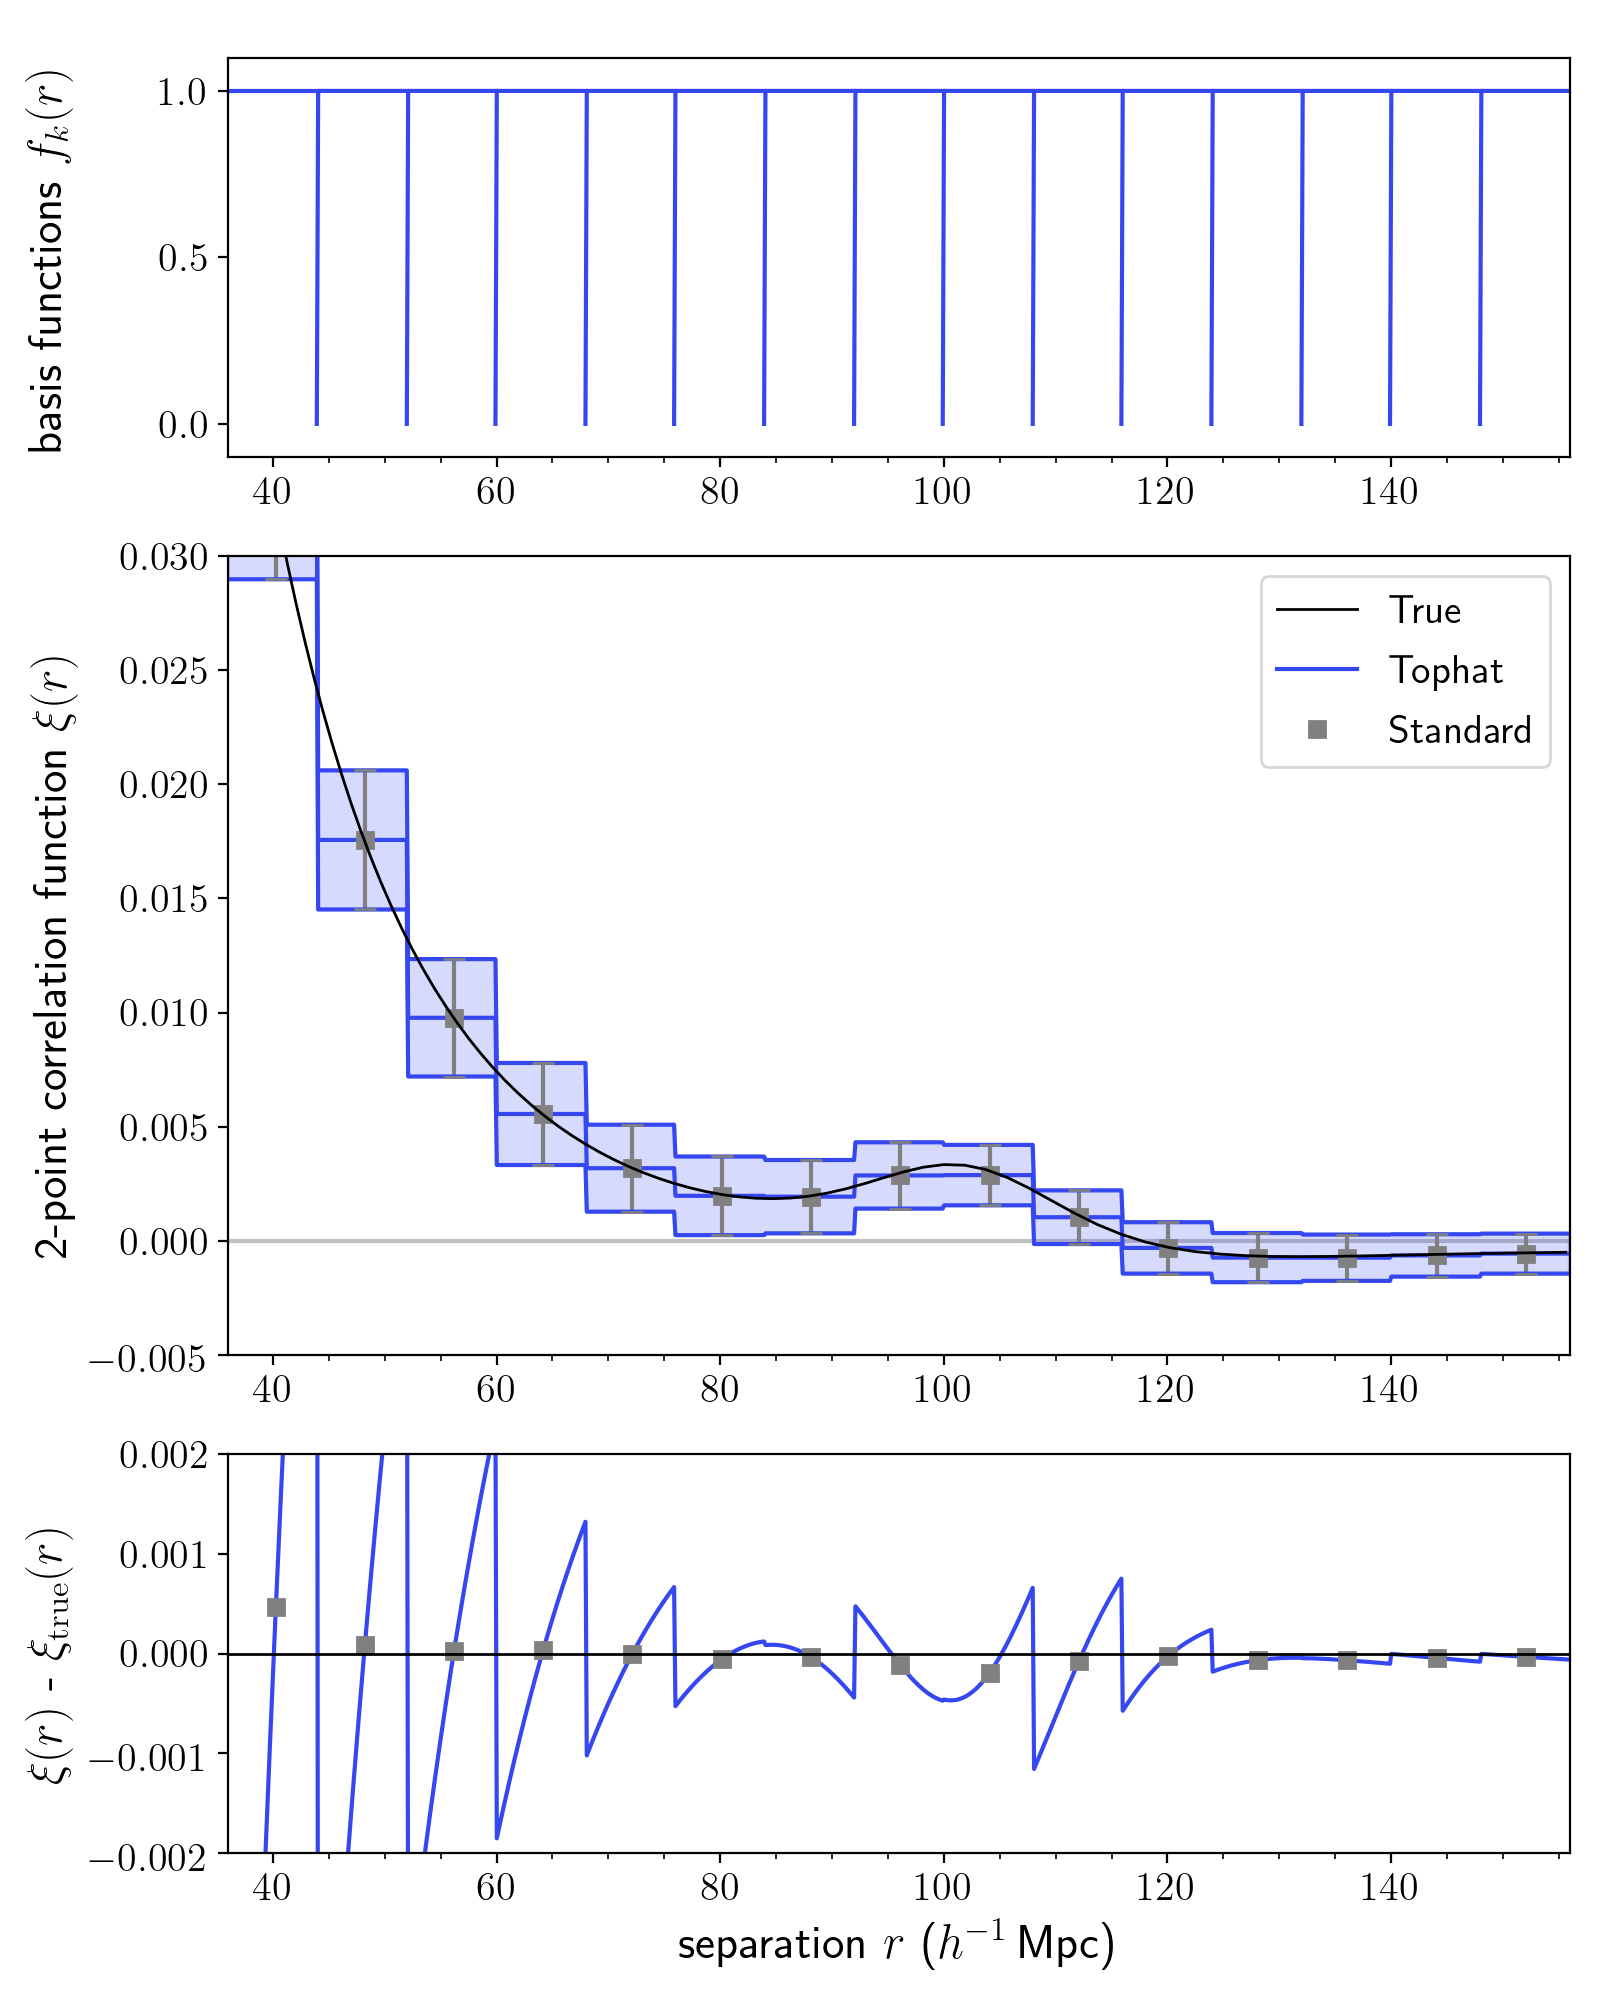
\includegraphics[width=0.8\textwidth]{xicomparison_2e-4_tophat8_theory8}
    \caption{A comparison between \est with a tophat basis (thin blue lines) and the standard estimator (grey squares). The top panel shows the basis functions used for the tophat estimator. The middle panel shows the mean of the estimated correlation functions for 1000 mock catalogs, compared to the true input \cf (thin black line); the shaded region and errorbars are the standard deviation of the \cf estimate. The lower panel shows the absolute error between the estimate and true \cf. \Est with a tophat basis is exactly equivalent to the standard estimator, but in a continuous form, emphasizing the fact that binning results in a poor representation of the true \cf.}
    \label{fig:tophat}
\end{figure}

\subsection{Demonstration using Spline Basis Functions}
\label{sec:spline}

\begin{figure}[ht]

\centering
    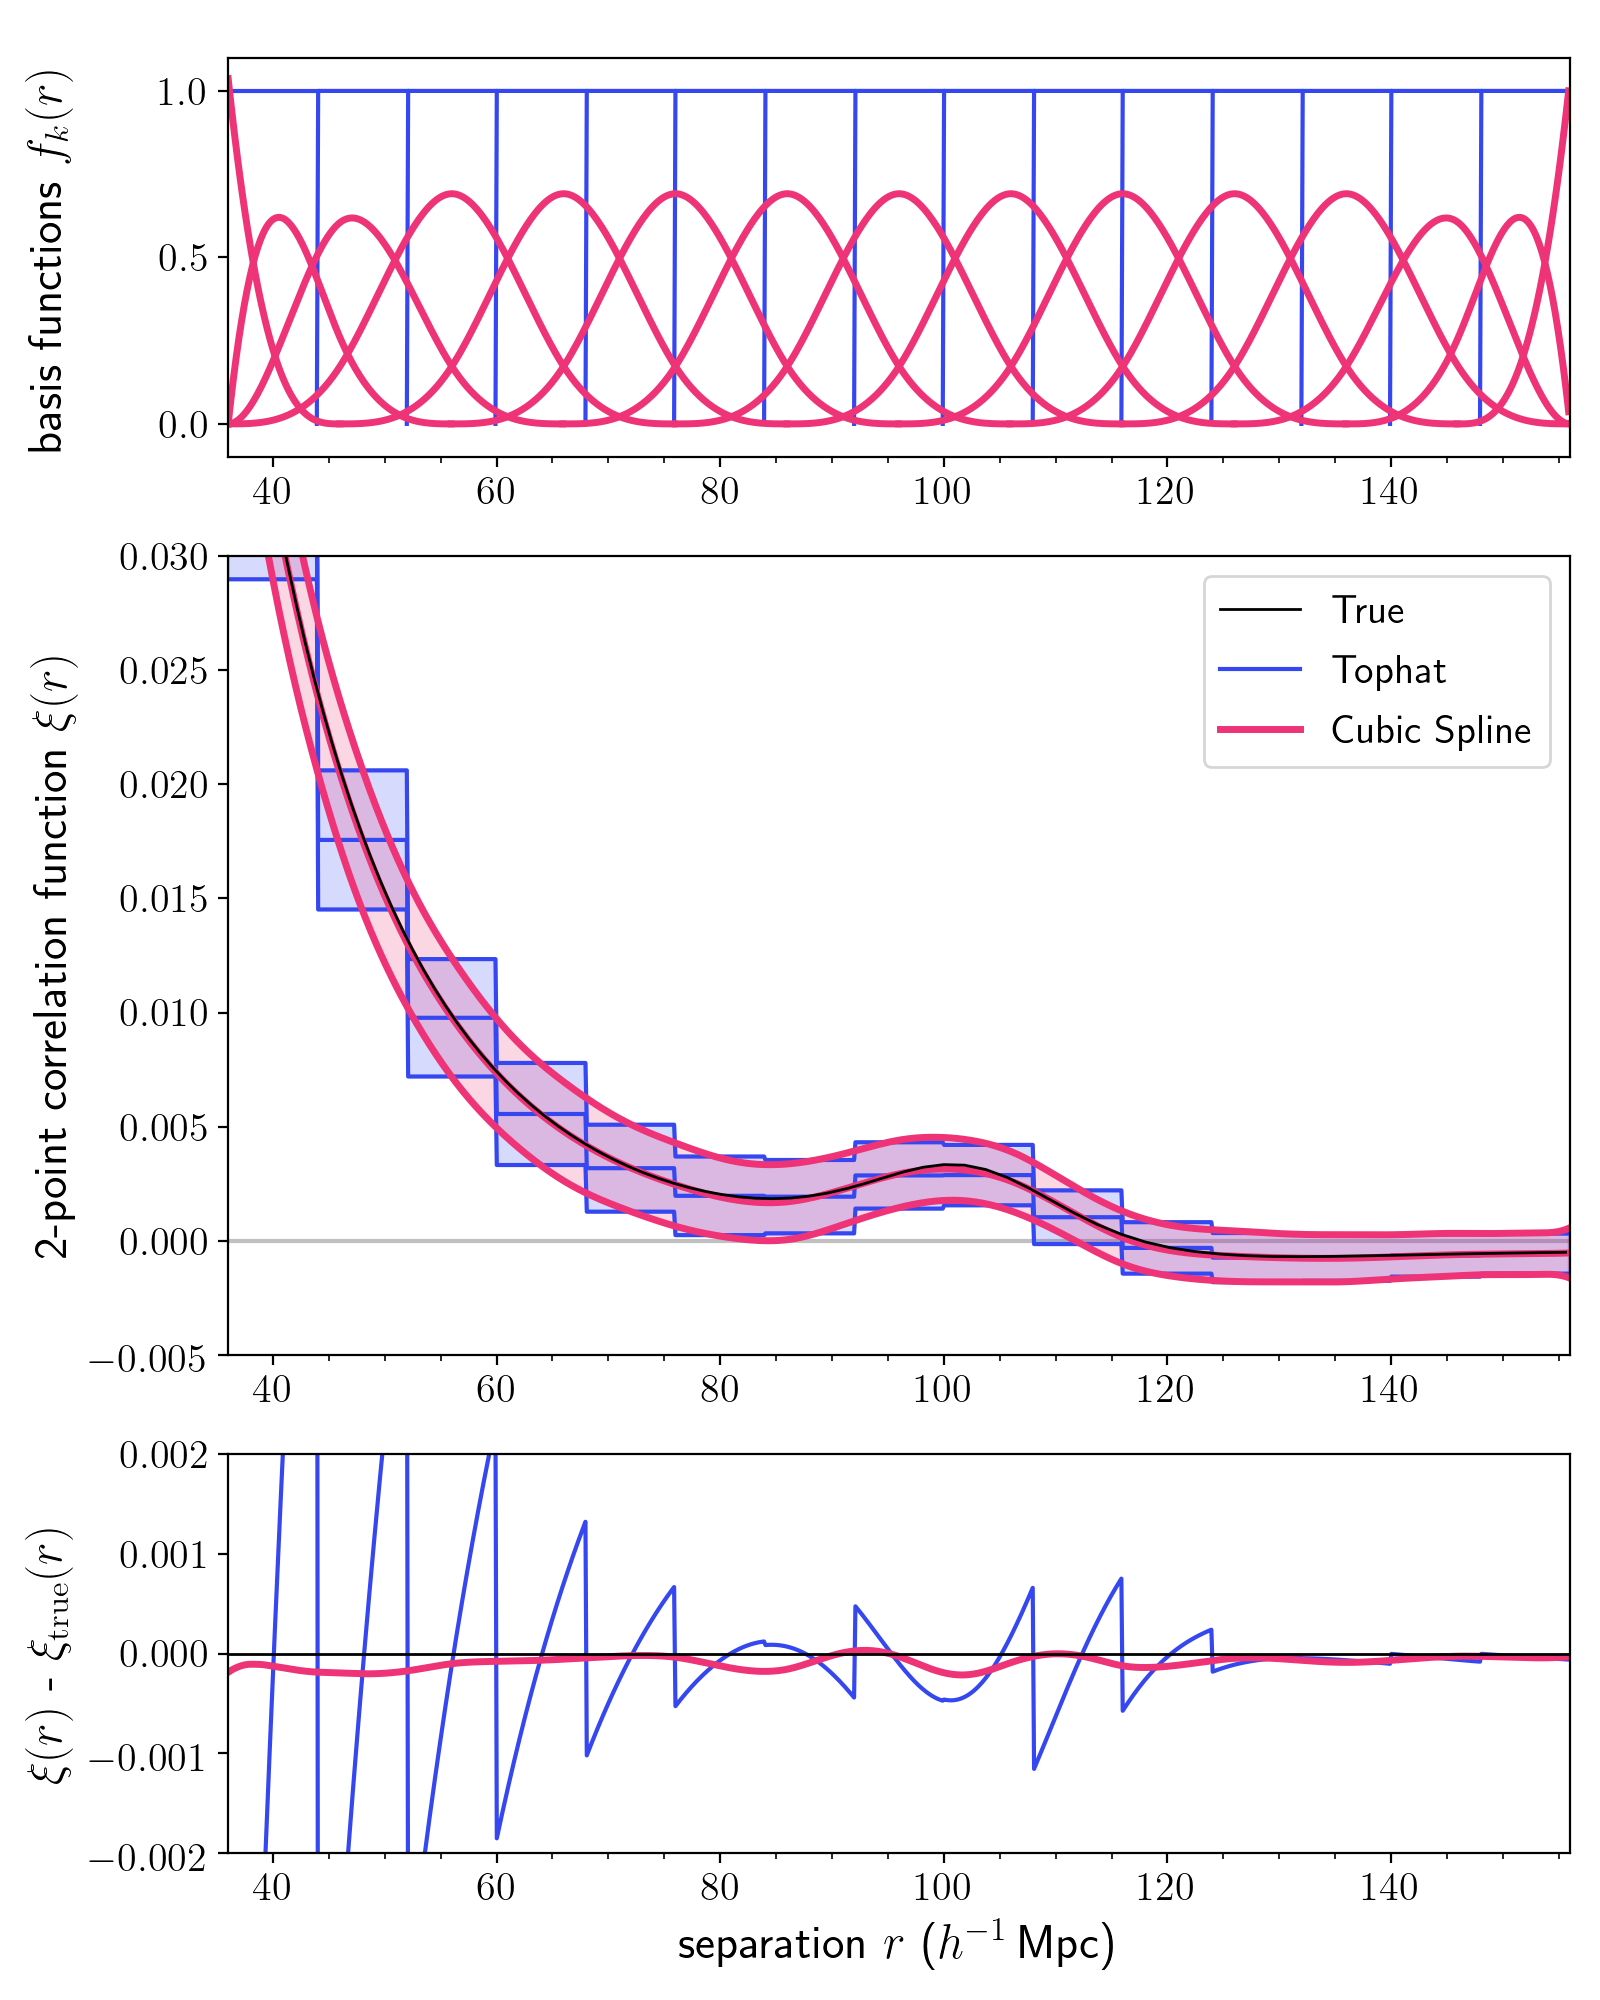
\includegraphics[width=0.8\textwidth]{xicomparison_2e-4_tophat8_spline}
    \caption{A comparison between \est with a cubic-spline basis function (thick red) and a standard tophat basis (thin blue). The top panel shows the basis functions used for each measurement. The middle panel shows the mean of the estimated correlation functions for each of the 1000 mock catalogs compared to the true input \cf (thin black); the shaded region is the standard deviation. The lower panel shows the absolute error between the estimate and true \cf. It is clear that the spline basis function results in a correlation function that is a better representation of the true \cf in its shape and smoothness.}
    \label{fig:spline}
\end{figure}

A natural extension of tophat basis functions is the B-spline.
B-splines of order $n$ are piecewise polynomials of order $n-1$; they constitute the basis functions for spline interpolation \citep{deBoor1987}.
They have the nice property that the functions and their derivatives can be continuous, depending on the order.
Further, B-splines are well-localized, which provides a more direct comparison to the typical tophat basis (which is entirely localized).
For this demonstration we use fourth-order B-splines, which constitute the set of basis functions for a cubic spline, as they are the lowest-order spline to have a continuous first derivative.

We compare the estimator with a cubic-spline basis to the standard estimator, reformulated as continuous functions using a tophat basis; the results are shown in Figure~\ref{fig:spline}.
The basis functions are shown in the top panel of the figure.
We use the same tophat basis as above.
For the cubic-spline basis, we use the same $r$-range and number of basis functions, and knots chosen to evenly span the range. 
The cubic-spline bases on the edge have different shapes such that they remain normalized; we note that generally, one should choose the basis functions such that the range of the \cf that is of interest does not depend on the range of the basis functions.

The estimator using the cubic-spline basis clearly produces a better fit to the true correlation function in its shape and smoothness at every point across the scale range, compared to the estimator using the tophat basis.
The bottom panel shows the error with respect to the truth; the cubic-spline estimator is more generally more accurate, and straightforward to compare to the truth (or model) at every scale.
On the other hand, in order to compare the binned correlation to a model, one must integrate the model over the bin range, though in practice the model is often just evaluated at the effective $r$ of each bin.
This comparison demonstrates that there exist other sets of basis functions that produce better representations of the data compared to the standard tophat/binned estimator.
The choice of a high-order spline may be useful for cases in which one wants a mostly localized yet representative estimate of the \cf, or smooth derivatives.
Generally, the choice of basis functions should be tailored to the scientific use case; in the next section we explore the case of a BAO analysis.


\subsection{BAO Scale Estimation Test}
\label{sec:bao}

The measurement of the baryon acoustic oscillation (BAO) scale provides an apt use case for our estimator.
The BAO feature is a peak in clustering on large scales, $\sim$150 Mpc ($\sim$100\hmpc), making it less sensitive to small-scale astrophysical effects.
It is one of the best tools for constraining cosmological models, in particular the distance--redshift relation \citep{Eisenstein2005, Kazin2010, Anderson2012, Anderson2014, Alam2016}.

We base our BAO analysis on the method of the BOSS DR10 and 11 analysis \citep{Anderson2014}.
We estimate the spherically averaged 3-dimensional correlation function, $\hat{\xi}(r)$, where $r$ is the separation between pairs.
(BAO analyses are typically done in redshift space, estimating $\hat{\xi}(s)$, where $s$ is the redshift-space separation between pairs, but here we are using a periodic box in which we know the true galaxy positions, so we just use the real-space distance $r$.)
In order to extract information about the baryon acoustic feature from galaxy clustering, we must choose a fiducial cosmological model to convert redshifts to distances.
If we choose an incorrect model, the scales in the power spectrum will be dilated, so the oscillation wavelength---and thus the BAO peak position---will be shifted.
We can model this shift as a scale dilation parameter, $\alpha$, which is a function of the relevant distance scales in the true and fiducial cosmologies, defined as
\begin{equation} \label{eq:alpha}
\alpha = \Bigg( \frac{D_\mathrm{A}(z)}{D_\mathrm{A}^{\text{mod}}(z)} \Bigg)^{2/3} \Bigg( \frac{H^{\text{mod}}(z)}{H(z)} \Bigg)^{1/3} \Bigg( \frac{r_\mathrm{s}^{\text{mod}}}{r_\mathrm{s}} \Bigg) ~,
\end{equation}
where $D_\mathrm{A}$ is the angular diameter distance, $H$ is the Hubble parameter, $z$ is the redshift, $r_\mathrm{s}$ is the sound horizon scale at the drag epoch, and the superscript ``$\text{mod}$'' denotes the value for the chosen fiducial model (the non-superscripted parameters are the true values).
Qualitatively, if the fit prefers $\alpha>1$, this suggests the true position of the BAO peak is at a smaller scale than in the fiducial model, whereas if $\alpha<1$, the peak is at a larger scale.
With isotropic analyses, there is a degeneracy between $D_\mathrm{A}$ and $H$, so typically a combination of these values is reported; the degeneracy can be broken with anisotropic BAO analyses.
Our estimator could straightforwardly perform an estimate of the anisotropic correlation function, but for demonstration purposes we perform an isotropic analysis here and focus on the recovered value of $\alpha$.

In standard practice, the fitting function used to determine the value of $\alpha$ is 
\begin{equation}
\xi^{\mathrm{fit}}(r) = B^2 \xi^{\mathrm{mod}}(\alpha r) + \frac{a_1}{r^2} + \frac{a_2}{r} + a_3 ~,
\end{equation}
where $B$ is a constant that allows for a large-scale bias, and $a_1$, $a_2$, and $a_3$ are nuisance parameters to account for the broadband shape.
A $\chi^2$ fit is performed with five free parameters: $\alpha$, $B$, $a_1$, $a_2$, and $a_3$. 
\KSF{TODO: KSF is figuring out how this actually done and flesh out this paragraph!}
The resulting value for $\alpha$ is used to derive the actual values of the distance scales of interest.
Typically, density-field reconstruction is performed before applying the estimator to correct for nonlinear growth around the BAO scale \citep{Eisenstein2007}; for our toy example, we omit this step.

The form of the standard fitting function is well-suited to our estimator, as it is a few-parameter model with a linear combination of terms.
To use our estimator to estimate $\alpha$, we add a term that includes the partial derivative of the model with respect to $\alpha$.
This allows us to have fixed basis functions, and for an initial choice of $\alpha_\mathrm{guess}$, determine the change in this value needed to improve the fit. 
Our fitting function is then
\begin{equation} \label{eq:baoiter_fit}
\xi^\mathrm{fit}(r) = B^2\,\xi^\mathrm{mod}(\alpha_\mathrm{guess}\,r) + C\,k_0\,\frac{\dd \xi^\mathrm{mod}(\alpha_\mathrm{guess}\,r)}{\dd \alpha} + a_1\,\frac{k_1}{r^2} + a_2\,\frac{k_2}{r} + a_3\,k_3 ~,
\end{equation}
where $C$ is an additional coefficient that describes the contribution of the derivative term, and $k_0$, $k_1$, $k_2$, and $k_3$ are constants that determine the initial magnitude of the basis functions.
In this case, the free parameters are $B^2$, $C$, $a_1$, $a_2$, and $a_3$.
Note that in theory the choice of $k_i$ values shouldn't matter as the estimator is affine invariant (see Appendix~\ref{sec:affine}), but in practice reasonable choices are important for stability.
The adopted $k_i$ values are noted in Appendix~\ref{sec:baoiter}.

To use the estimator for a BAO measurement, we input these five terms as the five basis functions of our estimator.
The estimator outputs an amplitude vector $\bld{a}$ as described in Section~\ref{sec:est}, which describes the contribution of each basis function---precisely the values of the free parameters, scaled by $k_i$.
From the value of $C$, we can determine our estimate of the scale dilation parameter, $\hat{\alpha}$, as $\hat{\alpha} = \alpha_\mathrm{guess} + C\,k_0$, based on the definition of finite derivatives. 
With this formulation, a value of $C=0$ indicates that the current $\alpha_\mathrm{guess}$ gives the best fit to the data (given the chosen cosmological model), while nonzero values give the magnitude and direction of the necessary change in the scale dilation parameter to optimally fit the data.
In practice, we apply an iterative procedure to converge at our best estimate $\hat{\alpha}$; this procedure and other implementation details are described in Appendix~\ref{sec:baoiter}.

\begin{figure}[ht]
\centering
    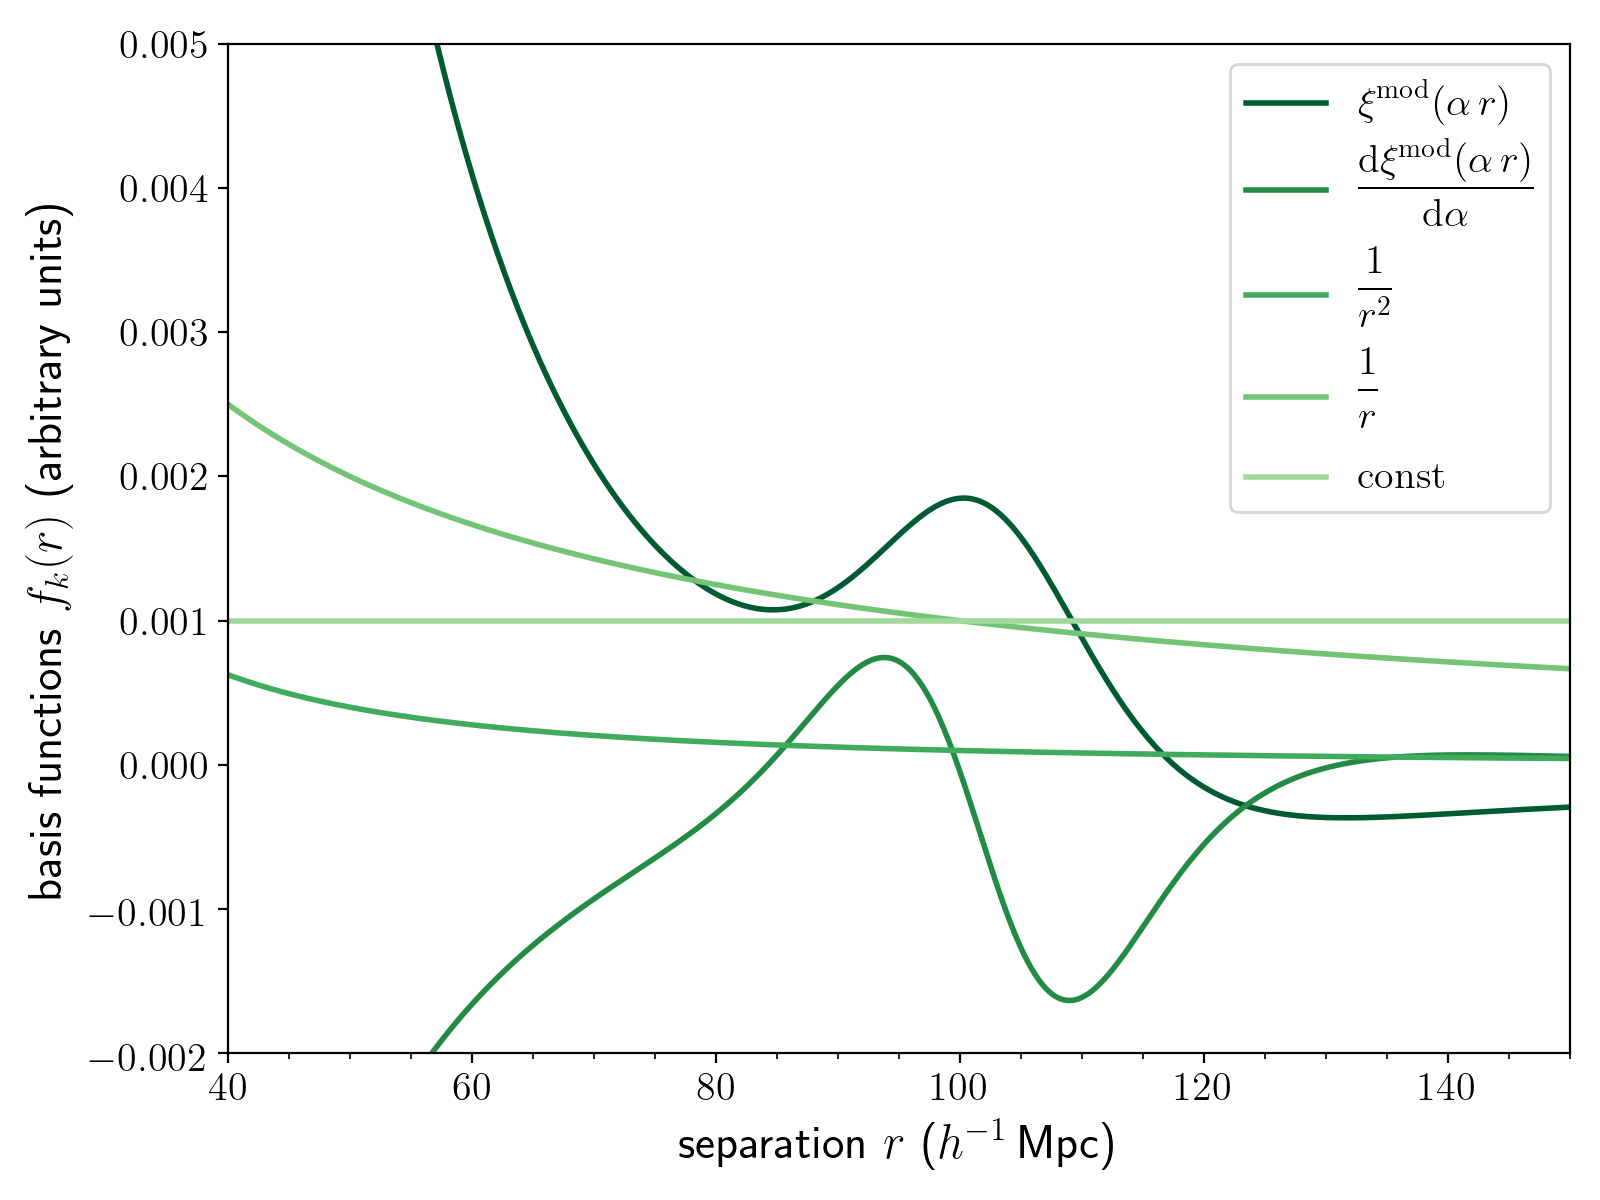
\includegraphics[width=0.8\textwidth]{bao_bases}
    \caption{The set of basis functions used to fit for the BAO scale using our estimator. The $\xi^\mathrm{mod}(\alpha\,r)$ term (darkest green) is the correlation function computed using fiducial model, with some scale dilation $\alpha$. The derivative term (second-to-darkest green) is the derivative of this model with respect to $\alpha$, which allows for the direct estimation of this parameter. The other three terms (lighter greens) are nuisance parameters to fit the broadband shape.}
    \label{fig:bao_bases}
\end{figure}

We demonstrate this method using our set of lognormal mock catalogs.
We construct a recovery test following that in \cite{Hinton2019}.
We assume the fiducial cosmological model used in \cite{Beutler2017}: $\Omega_{\text{m}} = 0.31$, $h = 0.676$, $\Omega_{\text{b}} = 0.04814$, $n_s = 0.97$. 
As we know the cosmology used for our mock catalogs, we can compute the true value of the scale dilation parameter, $\alpha_{\text{true}}=0.9987$.
(Here our choice of fiducial model happened to be close to the true model, so our $\alpha_{\text{true}}$ is very close to 1; this is typical, as our cosmological model is fairly well-constrained.)
With this fiducial model, we can construct the basis functions for our estimator; these are shown (with $\alpha=1$ and arbitrary scaling) in Figure~\ref{fig:bao_bases}.

We apply our iterative estimation procedure to each of the 1000 mocks; the mean of the resulting estimates for the correlation function is shown in Figure~\ref{fig:bao}.
We show the BAO basis functions in the top panel, as in Figure~\ref{fig:bao_bases}.
We compare \est using the BAO bases with that using tophat bases, as in the previous sections.
The correlation function estimated with the BAO bases clearly produces a more representative estimate at all scales.
The estimate is also smoother than that produced using the cubic-spline basis functions (Figure~\ref{fig:spline}).
More importantly, it is scientifically motivated: the estimator directly gives us the relative contributions of the terms of the BAO fitting functions.
Further, the BAO-based estimate requires only five components, while the tophat basis requires 15 components (or bins, in the standard approach) in the same scale range.
This is critical for the efficient computation of a precise covariance matrix, as the errors depend on the number of components used for the estimate, as described in Section~\ref{sec:covariance}.
\Est with the BAO basis functions could reduce the number of mocks needed to achieve the same precision by a factor of a few to an order of magnitude; as these expensive cosmological simulations are currently the limiting step in two-point analyses, this could be highly impactful.

\label{fig:bao}
\begin{figure}[th]
\centering
    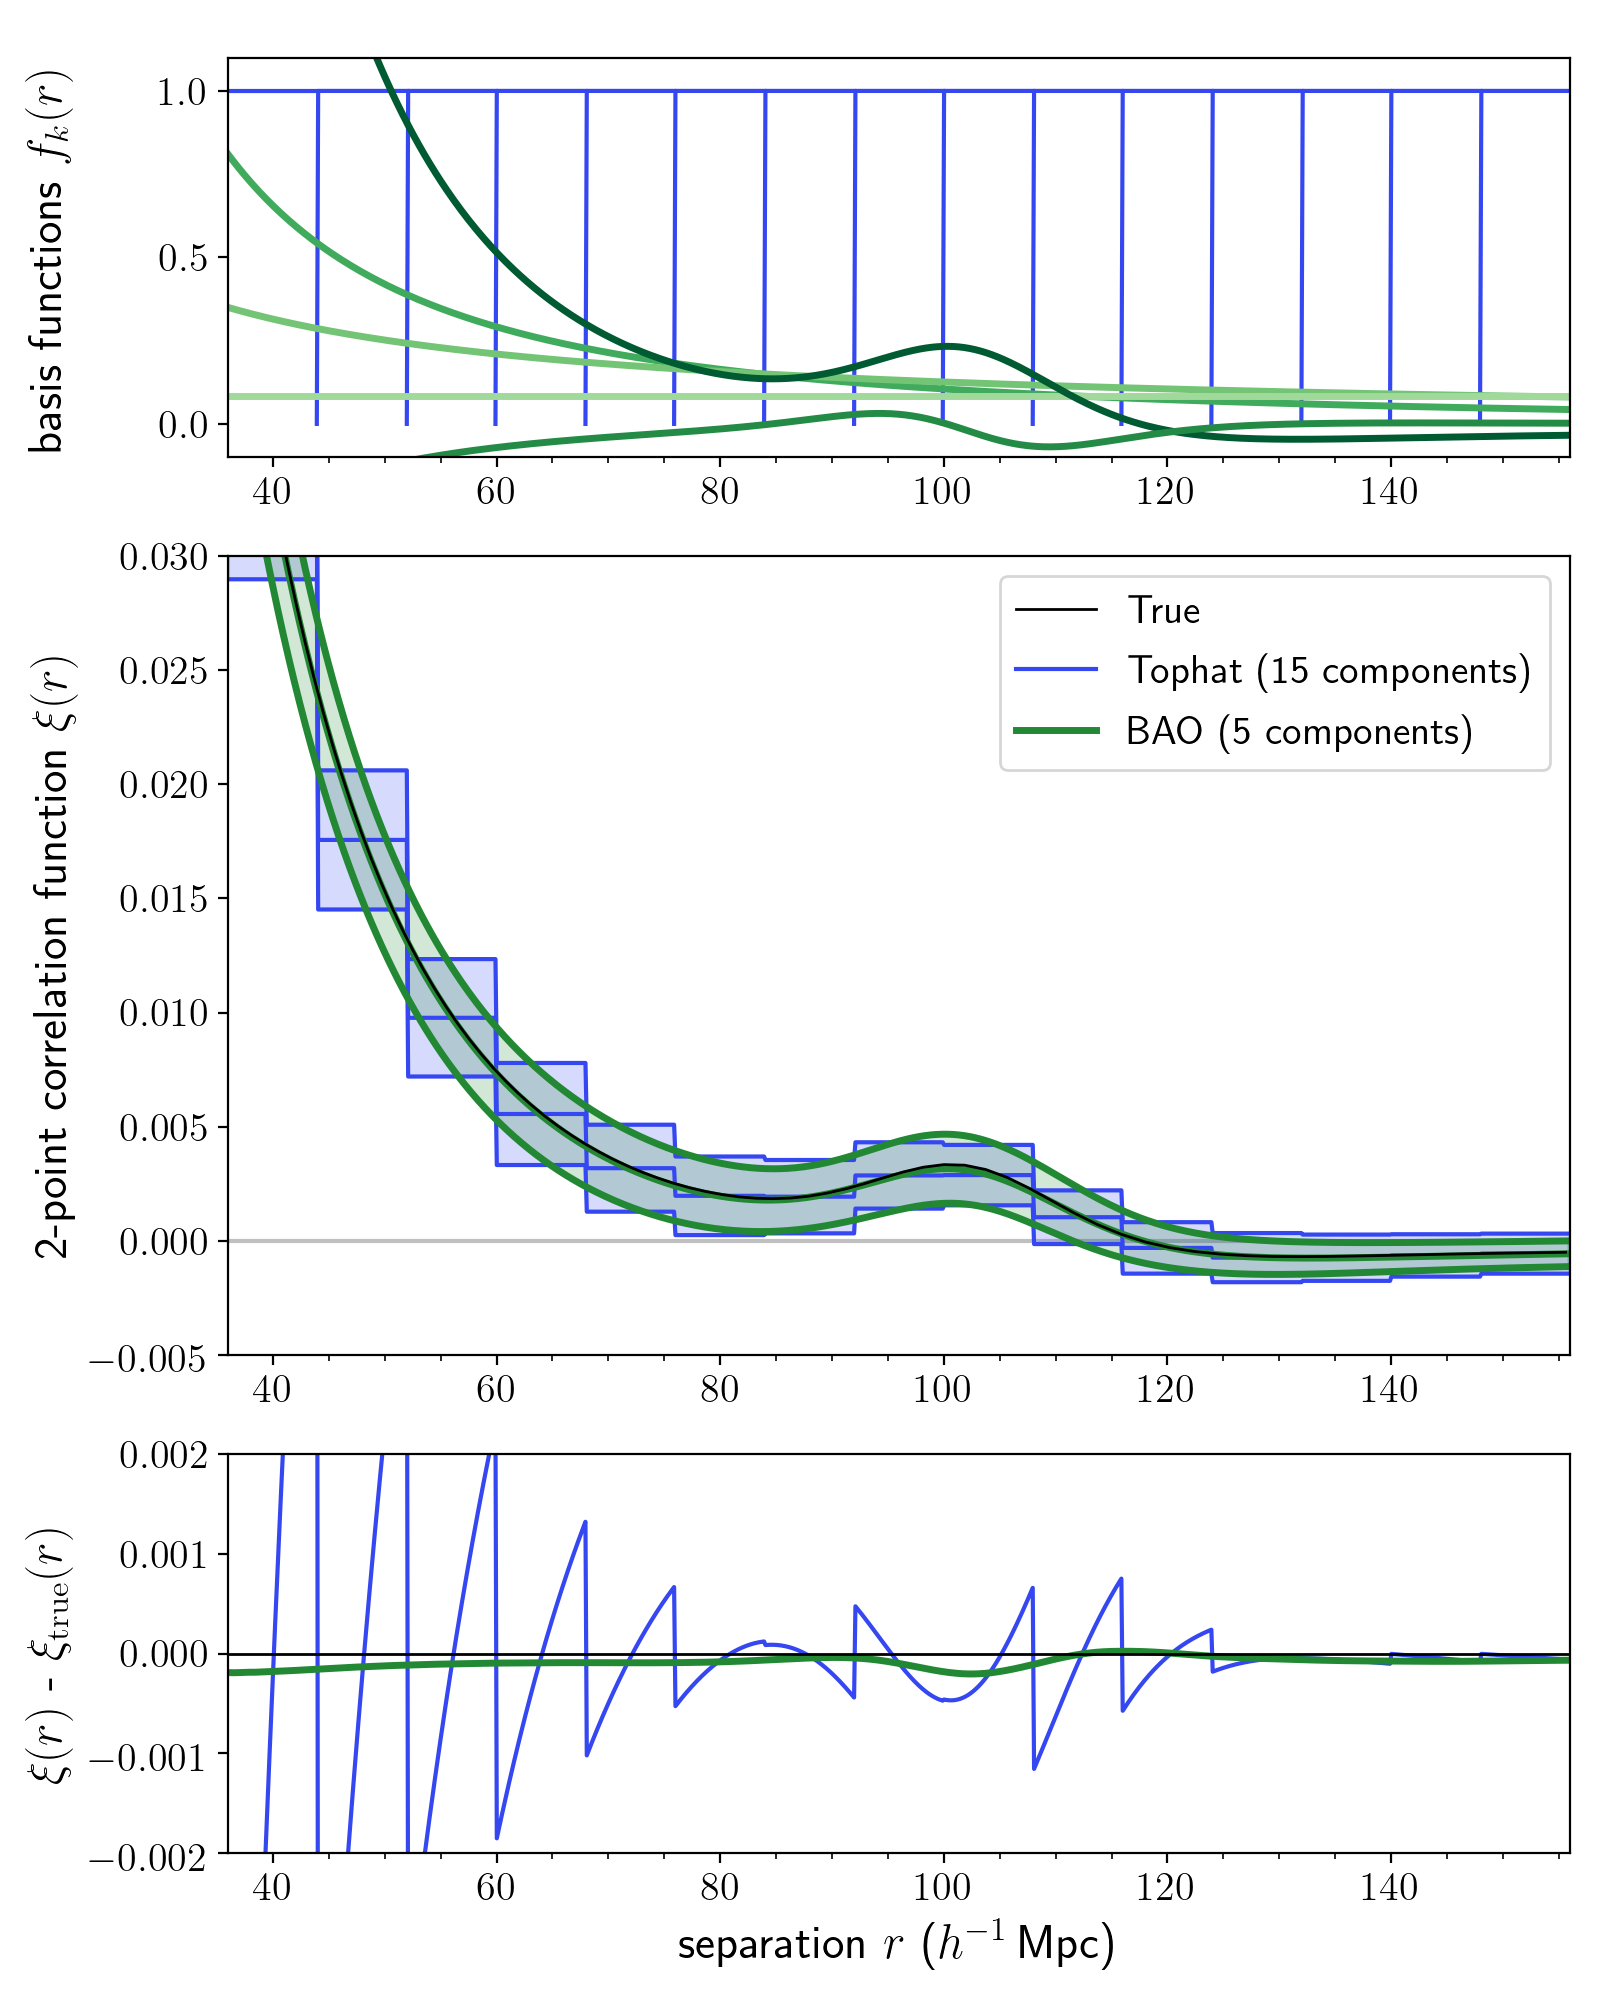
\includegraphics[width=0.8\textwidth]{xicomparison_2e-4_tophat8_baoiter}
    \caption{Estimation of the correlation function using our estimator with basis functions based on the BAO fitting function (thick green). The line is the mean of the final estimate from the iteration procedure for 1000 mocks, and the shaded region is the $1\sigma$ variation. We also show the standard Landy--Szalay estimator, displayed as a tophat function (thin blue), as well as the true input correlation function (thin black). The basis functions are the same as those shown in Figure~\ref{fig:bao_bases}, with arbitrary scaling.}
\end{figure}

We note that these basis functions are significantly different than the tophat or B-spline bases previously explored.
One important difference is that they are not localized.
This means that data at all scales could contribute to all basis functions.
It is then critical for the investigator to ensure that the range of scales chosen is reasonable for the scientific problem at hand and that the final estimate of the parameter of interest does not depend on the details of this choice.
The nonlocality also means that the covariance matrix between the components will have a very different structure than typical binned covariance matrices.
We return to this issue in Section~\ref{sec:covariance}.

\KSF{I will flesh out the following paragraph once I perform the traditional method!}
\Est with the BAO bases gives us an estimate for $\alpha$ for each of the 1000 mock catalogs.
These are shown in comparison with the values estimated using the traditional fitting approach in Figure ZZZ. \KSF{update} 
The methods produce similar values of $\alpha$ \dots 
The mean estimate of the recovered scale dilation parameter is $\alpha=XXX \pm YYY$, very close to the true value of $\alpha = 0.9987$.
The mean estimate using the traditional approach is $\alpha=XXX \pm YYY$.
Our estimate is more accurate and precise \dots 


\section{Discussion} \label{sec:discuss}

\subsection{Summary of Results and Limitations}

This \documentname presented a method to estimate the two-point correlation function without the need for binning.
It generalizes the standard \cf estimator in a manner inspired by least-squares fitting: \est projects the data onto a set of user-chosen basis functions, and applies a normalization based on a random catalog.
Using a set of artificial mock catalogs, we showed that our method exactly reproduces the results of the standard approach with the choice of tophat basis functions, but in a way that demonstrates what the estimator is really measuring, namely a constant amplitude of clustering at every point within a radial separation bin.
\Est, however, has the capacity to be much more expressive than the standard estimator with a different choice of basis functions.
We demonstrated its use with cubic-spline basis functions, which results in a correlation function estimate that is much more representative of the expected shape and smoothness of the \cf.
Further, \est can be tailored to the scientific use case; we apply to it a toy baryon acoustic feature analysis, choosing basis functions to be the terms of a modified BAO fitting function.
This produced an estimate of the \cf that inherently reflects our beliefs about its form, and allowed us to directly estimate the scale dilation parameter with improved accuracy and precision compared to the standard estimator. \KSF{UPDATE this last line when analysis is done.}

While these are just a few example applications of our estimator (for others see Section~\ref{sec:applications}), they demonstrate the problems solved and opportunities created with \est.
In getting rid of the need for binning, the estimator can produce a much more \textit{representative} correlation function; a mixture of tophats is a very poor representation of the \cf. 
We almost always expect some sort of continuity in the functions we work with; nature does not bin.
In principle, one can ``avoid binning'' by working in the limit of infinitesimal bins.
This would, however, be impossible in the current framework of the \LS estimator and using mocks to perform uncertainty estimation.
In some sense, our method can be seen as effectively working in the limit of infinitesimal bins, but where those bins have been projected onto continuous functions.

One of the problems with binning is that there are choices to be made in bin widths and locations.
We note that our approach does not actually help these choice issues.
In fact, \est expands investigator choice almost infinitely, as the space of possible basis functions is far larger than the space of possible binnings.
That said, since the selection of basis functions can be designed for the science case at hand, the choices can be better motivated and lead directly to the final estimate one in which one is interested (e.g., our BAO estimate in Section~\ref{sec:bao}).  

Our approach does have certain limitations.
One restriction is the fact that the \cf forms of interest must be representable in terms of a linear combination of basis functions; this makes \est less appropriate in the case of nonlinear models.
The estimator must also evaluate the basis functions for every pair of objects, so highly complex functions may become intractable.
Finally, our estimator inherits many of the limitations of the Landy--Szalay estimator, including the fact that it contains a bias on clustered data and has non-optimal variance properties.
However, \est is further generalizable to other forms of the estimator (Section~\ref{sec:beyondls}), so in principle there is a formulation that further ameliorates these \LS-related limitations.

\subsection{Relationship to Other Modifications of \cf Estimators}
\label{sec:otherest}

On the surface, \est appears similar to other two-point function projects, including kernel density estimators \citep {Hatfield2016} and the marked correlation function \citep{Beisbart2000}.
While these formulations look similar, ours solves a different problem than these estimators.

Kernel density estimation (KDE) is a class of methods for estimating a probability density function from a set of data.
KDE methods essentially smooth the data with a given kernel, often a Gaussian.
This is useful when we want to reconstruct a distribution without making many assumptions about the data, as is required in parametric methods.
KDEs have found use in many areas of astrophyics, for example to measure the 21cm power spectrum with reduced foreground contamination \citep{Trott2019}, and to estimate luminosity functions with superior performance compared to binned methods \citep{Yuan2020}.
\cite{Hatfield2016} uses a KDE approach to estimate the angular correlation function, in order to address the issues of information loss and arbitrary bin choice inherent to binning; they optimize for the kernel choice, and find a correlation function consistant with that of the binned method.

Specifically, kernel density estimators take the contribution of each data point to be a kernel function centered on that value, and sum these to determine the full distribution.
In contrast, \est projects each data point onto fixed basis functions, which are distinct from the typical understanding of kernels.
As such, our estimator is not smearing out the data, as KDEs do; it is using the data to directly infer the contribution of each basis function.
This preserves the information in the data to the degree given by the chosen set of basis functions, which can in fact enhance features rather than smooth them.
More importantly, \est hinges on the $\TT{RR}\inv$ factor that rescales the data projection, resulting in a estimate that is closely related to a least-squares fit of the data.
This is very different from KDE methods, which in most contexts result in a strongly biased estimate, because it smooths the function over the width of the kernel.

Another method that shares similarities with \est is the marked correlation function (MCF, \citealt{Beisbart2000}; \citealt{Sheth2005}).
This estimator weights the two-point statistic by ``marks,'' which are typically properties of the tracers.
The MCF is useful for studying the connection between galaxies and their spatial clustering.
\cite{Skibba2006} used it to determine that luminosity-dependent clustering is a straightforward consequence of mass dependence.
\cite{Armijo2018} applied the MCF to test a class of modified gravity theories by marking with local density, demonstrating that there is additional information in the environmental dependence of clustering.
The MCF has also been shown to break the degeneracy between halo occupation distribution parameters and the cosmological parameter $\sigma_8$ \citep{WhitePadmanabhan2009}.

\Est can easily incorporate the \textit{idea} behind marks by choosing the basis functions to be functions of the desired properties of the tracer in addition to pair separation.
Combined with the choice of tophat basis functions and proper normalization, this would indeed be closely related to the measurements that can be made by the MCF.
However, \est can generalize this concept even further. 
Rather than still producing a two-point function that is only a function of separation, weighted by the marks, our estimator can elevate the marking properties to another continuous axis.
That is, it can estimate a multi-dimensional correlation function as a function of both separation and the given property.
This provides a more flexible way to look at the dependence of the \cf on the property, and has similar applicability to breaking parameter degeneracies.
We elaborate on the use cases for incorporating further tracer information into the choice of bases functions in Section~\ref{sec:applications}.


\subsection{Beyond the Landy--Szalay Estimator}
\label{sec:beyondls}

While we have formulated our estimator as a generalization of \LS, as this is the standard used in \cf analyses and has optimal properties under certain conditions, we can also reformulate it for other estimators.
Our formulation currently requires a normalization term (i.e. denominator) based on the random--random counts; for \LS we replace this with our $\TT{RR}$ term (\eqt{eq:qq_proj}).
This is also the case for the \cite{PeeblesHauser1974} (natural) estimator and the \cite{Hewett1982} estimator:
\begin{eqnarray}
    %using text so hyphens show up properly
    \bld{\hat{\xi}}_\text{P-H} &=& \frac{\vv{DD} - \vv{RR}}{\vv{RR}} \rightarrow \TT{RR}\inv \cdot \left( \vv{DD} - \vv{RR} \right)\\
    \bld{\hat{\xi}}_\text{Hew} &=& \frac{\vv{DD} - \vv{DR}}{\vv{RR}} \rightarrow \TT{RR}\inv \cdot \left( \vv{DD} - \vv{DR} \right) ~.
\end{eqnarray}
We can also straightforwardly generalize estimators which have a data--random cross-correlation as the normalization term, such as the \cite{DavisPeebles1983} estimator,
\begin{equation}
    \bld{\hat{\xi}}_\text{D-P} = \frac{\vv{DD} - \vv{DR}}{\vv{DR}} \rightarrow \TT{DR}\inv \cdot \left( \vv{DD} - \vv{DR} \right) ~,
\end{equation}
where we define
\begin{equation}
    \TT{DR} = \frac{2}{\NN{D}\,\NN{R}} \sum_{n} \sum_{m} \ff(\GG{n m}) \cdot \ff\T(\GG{n m}) ~.
\end{equation}

The continous form of these estimators can be extended to cross-correlations in the straightforward way expected.
This formulation could also be extended to nearly any linear combination of pair counts.
The estimator of \cite{VargasMagana2013}, for instance, selects the optimal combination of pair counts; our estimators could be combined to create an even more generalized estimator.
However, some estimator formulations use powers of these terms that are nontrivial to reformulate as normalization tensors for our estimation approach; we leave this problem for furture work.


\subsection{Implementation and Computational Performance}
\label{sec:comp}

We implement \est within the widely used correlation function package \texttt{Corrfunc} \citep{Sinha2019}.
In some sense, the most important implementation note is that we are capitalizing on all of the good engineering in Corrfunc that produces very fast pair identification. \KSF{TODO: reword}
The package is written in C with python bindings and utilities.
For every computation of the pair separation, we additionally pass the separation and any additional tracer information to the user-defined basis function.
We output the traditional pair counts as well as our component vector and, if desired, the component tensor.

The computational scaling for our estimator is by definition the same as the traditional method, as pair-finding remains the limiting factor.
However, because \est must evaluate the set of basis functions for each pair of galaxies, it can take longer.
For simple basis functions like splines, this will only marginally decrease performance.
For more complicated functions, \est may incur significant extra computational expense.
Basis functions can also be input on a grid (of separation or any other property) and then interpolated; the performance is then similar for all functions, depending on how the interpolation is done, but interpolating each function for each pair does somewhat decrease the performance.
Though the performance at the time of estimation may be slower than the traditional estimator, the choice of basis may significantly save computational time in other areas, such as reducing the number of mock catalogs required for covariance matrix estimation; see Section~\ref{sec:covariance}.

We detail a number of implementation choices here.
Our formulation of \est requires the inverse of the random--random tensor $\TT{RR}$ to compute the amplitudes (\eqt{eq:amplitude}).
However, we don't compute this inverse directly, as can be unstable, and is not in fact the end result we are interested in: we want the dot product between $\TT{RR}\inv$ and the numerator $\vv{}$ of the estimator.
For this reason, we use the ``solve'' operation which computes the solution $\bld{a}$ of the well-determined matrix equation $\TT{RR}\,\bld{a}=\bld{v}$.
We also make sure to report the condition number of the tensor, as numerical precision decreases as the condition number rises.
If the condition number large, then a rescaling of the basis functions or a rotation in the basis space can improve stability.


\subsection{Effect on Covariance Matrix Estimation}
\label{sec:covariance}

We have shown that \est results in \cf estimates that are just as accurate as binned estimates, with fewer components.
This is critical when estimating the covariance matrix, which is required for standard parameter inference.
The covariance matrix is difficult to compute analytically, though there is promising progress on this front (e.g., \citealt{Wadekar2020}).
For major analyses, it is usually estimated by evaluating the \cf on a large number of mock catalogs and computing the covariance between the bins (e.g., \citealt{Reid2010}; \citealt{Anderson2014}).
The unbiased estimator for the sample covariance matrix is (e.g., \citealt{Anderson2003})
\begin{equation}
%using \big and \bigg instead of \left and \right because the different sides give different sizes with the latter two
\big[ \bld{\hat{C}}^\mathrm{ML} \big]_{ij} = \frac{1}{\NN{mocks}-1} \sum_{q=1}^{\NN{mocks}} \bigg( \big[\bld{\xi}_q \big]_i - \bar{\bld{\xi}}_i \bigg) \bigg([\bld{\xi}_q \big]_j - \bar{\bld{\xi}}_j \bigg)\T ~,
\end{equation}
where $q$ denotes the index of the mock, $i$ and $j$ denote the index of the bin or component, $\bld{\xi}$ denotes the estimate in that bin for that mock, and $\bar{\bld{\xi}}$ denotes the mean value of the estimate in that bin across the mocks, where we have omitted the hat for clarity.

We typically require the inverse covariance matrix for analyses, but its form is nontrivial, as the inverse of an unbiased estimator is not necessarily unbiased.
Standard practice applies a correction factor \citep{Hartlap2007},
\begin{equation}
\bld{\hat{C}}\inv = \frac{\NN{mocks}-\NN{bins}-2}{\NN{mocks}-1} \left( \bld{\hat{C}}^\mathrm{ML} \right) \inv ~.
\end{equation}
However, this does not correct for errors in the covariance matrix; these propagate to errors on the estimated cosmological parameters, resulting in an overestimation of the error bars (\citealt{Hartlap2007}; \citealt{Dodelson2013} \citealt{Percival2014}; \citealt{TaylorJoachimi2014}).
Assuming that $\NN{mocks} >> \NN{bins}$ (with both much larger than the number of parameters to be estimated), and that the measurements are Gaussian distribued, the error bars are inflated by a factor of $(1 + \NN{bins}/\NN{mocks})$ (i.e., the true constraints are tighter than the derived ones).
This factor becomes critical at the precision of cosmological parameter estimation \citep{Percival2014}.

Typically, this is dealt with by generating a very large number of mocks.
For the Baryon Oscillation Spectroscopic Survey (BOSS, \citealt{Dawson2013}) DR9 analysis, 600 mocks were needed and the two-point correlation function used 41 bins \citep{Sanchez2012} (though they also perform a restricted 15-bin analysis over the BAO peak scales). 
For the BOSS DR14 fiducial \cf results, 1000 mocks and 18 bins were used \cite{Ata2017}.
Some surveys have already turned to approximate methods for these mock catalogs instead of performing full cosmological simulations, as the cost is prohibitive.
Future surveys will have even more costly requirements on mock catalogs, with larger simulations necessary to cover the larger survey volumes and more realistic mocks required to achieve the desired accuracy and precision on the covariance matrix.

% Our estimator can significantly lower these requirements by 
% \KSF{I went down some rabbit holes trying to find the numbers for DES and other surveys, it's not as clear. Is it ok as is or should I keep digging?}
% \KSF{it turns out that at least for DR14, some approximate method was used, so they weren't full cosmo sims and didn't take that long. should i try to figure out which analyses still used/use full sims to cite? any leads here?}
% \KSF{surveys are thinking about approximate mocks and different strategies, but they could change the number of mocks needed over night by changing the number of basis. if mocks are good enough, then just get a more accurate estimate.}

An alternative to increasing $\NN{mocks}$ is decreasing $\NN{bins}$ to achieve the same error on precision.
In the binned standard method, this is shown to \emph{increase} the statistical variance, albeit only slightly \citep{Percival2014}.
A substantial increase in bin width would prevent capturing information in finer clustering features; even the relatively broad BAO peak requires a bin size on the order of its width of $\sim$10\hmpc.
In fact, in the standard method more bins would typically be desireable, but the number is limited by the available number of mocks for covariance matrix computation.

We have shown that we can use \est to estimate the \cf using fewer components, without sacrificing accuracy.
This means that we can safely reduce $\NN{bins}$, or in our case, the number $K$ of components (or basis functions).
The covariance matrix will then express the covariance between these components (rather than bins, as we have obviated binning).
To then achieve the same precision on the error on the cosmological parameters, a lower value of $\NN{mocks}$ becomes possible.
This will significantly reduce requirements on mock catalog construction, which will be particularly important for upcoming large surveys. 
Alternatively, with the same number of mock catalogs, one can achieve increased precision just using \est as an alternative to the standard estimator.

Another issue with the covariance of the standard estimator is that the uncertainty is highly correlated across bins.
Thus the diagonal terms of the covariance matrix are poor representations of the true error on each bin.
The errors can be decorrelated by choosing a new estimator that is a linear combination of the original \cf bins. 
\cite{Hamilton2000} proposed a transformation using the symmetric square root of the Fisher matrix, and this was shown in \cite{Anderson2014} to significantly suppress the off-diagonal elements of the covariance matrix.
While this decorrelated covariance matrix is not used in the fitting in that analyses, it is useful for visualizing the uncertainty of the \cf estimates.
\Est could also be used to obtain a decorrelated covariance matrix.
One could perform an initial estimation with standard bins or basis functions, and then apply a transformation to decorrelation them.
These decorrelated bins could then be passed to the estimator as basis functions, and the analysis run again, in order to obtain a direct estimation that produces representative diagonal errors.
This might be particularly important for unlocalized basis functions such as the BAO basis functions, which are expected to have highly correlated errors.
Any covariance estimate will have to estimate these covariances well, but of course this is also true for the tophat basis where the covariances are nontrivial.

\subsection{Further Applications}
\label{sec:applications}

The formulation of \est opens up many possibilities for extracting information from the correlation function.
The most straightforward applications are standard basis functions or linearizeable astrophysical models, as we have shown for the standard BAO fitting function (Section~\ref{sec:bao}).
Other applications for the direct estimation of cosmological parameters could include the growth rate of cosmic structure $f$ \citep{Satpathy2016, Reid2018} and primordial non-Gaussianity in the local density field $f^{local}_{NL}$ \citep{Karagiannis2014}.

One could take this idea even further by choosing as basis functions a parametrized model of the \cf and the derivatives of this model with respect to the parameters of interest, such as cosmological parameters or halo occupation distribution parameters.
\Est would then directly output the projection of the \cf onto the derivative terms, which would then be translatable to changes in the  model that best fits the data.
This is analogous to the BAO analysis performed in Section~\ref{sec:bao}, but with a higher-dimensional space of derivatives of parameters of interest.
This approach would essentially perform a direct estimation of the parameters, without the need for the intermediate steps of binning and fitting.

Another class of applications involves a choice of basis functions that depend not only on the separation between tracer pairs, but also on the properties of the tracers themselves.
One such use case is the redshift dependence of the Alcock--Paczynski effect \citep{AlcockPaczynski1979}, which can be used to constrain the matter density $\Omega_m$ and the dark energy equation of state parameter $w$ \citep{Li2016}.
The basis functions $f$ in this case would take the form
\begin{equation}
    \label{eq:ff_redshift}
    \ff_k(\GG{n n'}) = \ff_k(|\bld{r}_n - \bld{r}_{n'}|, z_n, z_{n'}) ~,
\end{equation}
where $z$ is the redshift of tracer $n$ or $n'$.
\Est would then output a \cf that is a function of both separation and redshift, providing a continuous way to look at the redshift dependence of clustering.

This approach would also lend itself to analyzing how the LSS relates to galaxy formation, a connection critical for understanding this astrophysical process.
The traditional way of doing this involves binning by galaxy luminosity, and then computing the correlation function of the galaxies in each bin (e.g., \citealt{Budavari2003}, \citealt{Zehavi2011}, \citealt{Durkalec2018}).
\Est can remove the need for this extra layer of binning by using basis functions that depend on both the pair separation and on some function of the luminosities of the two galaxies.
Similarly to the example of redshift dependence in \eqt{eq:ff_redshift} above, in this case the data payload $\GG{n n'}$ would contain the galaxy luminosities $L_n$ and $L_{n'}$ in addition to the pair separation $|\bld{r}_n - \bld{r}_{n'}|$, and the basis functions $\ff_k$ would take all of these as parameters.
This would result in a direct way to look at the \cf luminosity dependence.
This could be extended to other galaxy properties, such as color or Hubble type (e.g., \citealt{Li2006}, \citealt{Skibba2014}), as well as environmental properties like the local density (e.g., \citealt{Abbas2006}).
\Est provides the flexibility to explore such a high-dimensional parameter space, while binned methods become quickly limited by number statistics as one tries to include more parameters.

Beyond these standard use cases, the estimator gives us the opportunity to investigate more subtle or exotic signals which are anomalous with respect to our conventional models.
Anomalies could appear as inhomogeneities or anisotropies in the data.
For example, \cite{MukherjeeWandelt2018} investigated whether there is a directional dependence in estimated cosmological parameters across the sky, by performing analyses on patches of the Cosmic Microwave Background.
Another possibility is anisotropy in the cosmic acceleration, which could leave signatures in measurements made using various phenomena including baryon acoustic oscillations \citep{Faltenbacher2012} and Type Ia supernovae \citep{Colin2019}.
With our estimator, we could introduce a dependence on location or direction into our basis functions, and constrain the potential deviation from homogeneity or isotropy.
\Est would allow for a more precise estimate of this dependence as it doesn't require any sort of patches or spatial binning, instead estimating a multi-dimensional continuous \cf.
While these effects would be highly degenerate with systematics, our estimator combined with robust systematics mitigation opens investigation channels into new physics.

Finally, our estimator can be directly related to a power spectrum analysis.
We could choose a Fourier basis as our set of continuous functions.
This would allow us to directly project the data onto Fourier modes.
This represents a step towards unifying the correlation function and the power spectrum.


\acknowledgements
KSF was supported by the NASA FINESST grant [grant number] \KSF{FILL OUT} during the completion of this work.
The authors thank Jeremy Tinker and Michael Blanton for helpful insights, and the members of the Flatiron Astronomical Data Group for useful feedback.
KSF would like to acknowledge significant code feedback and support from Manodeep Sinha and Lehman Garrison.
KSF also thanks Roman Scoccimarro, David Grier, Alex Barnett, Lucia Perez, James Rhoads, Sangeeta Malhotra, Drew Jamieson, and Chris Lovell for helpful discussions.
All of the code used in this \documentname is available open-source at \texttt{github.com/kstoreyf/Corrfunc} and \texttt{github.com/kstoreyf/continuous-estimator}. 

\appendix
\section{Affine Invariance of the Estimator}\label{sec:affine}

The estimate of the \cf with \est should not depend on the scaling of the chosen basis functions.
Thus we expect \est to be invariant under affine transformations of the basis functions, meaning transformations that preserve collinearity and distance ratios; the following demonstrates this affine invariance.

We represent the affine transformation by an invertible transformation matrix $\bld{M}$ that modifies the basis functions $\ff$, such that 
\begin{equation}
\ff' \leftarrow \bld{M}\,\ff ~,
\end{equation}
where the prime indicates our affine-transformed basis.
We choose $\bld{M}$ to be invertible to ensure the two bases have the same expressive capacity.
Then in the primed basis, the pair counts become
\begin{eqnarray}\displaystyle
\vv{DD}' &=& \adjustlimits \sum_{n} \sum_{n'} \ff_{n n'}' = \sum_{n n'} \bld{M}\,\ff_{n n'} = \bld{M}\,\vv{DD}
\\
\vv{DR}' &=& \sum_{n} \sum_{m} \ff_{n m}' = \sum_{n m} \bld{M}\,\ff_{n m} = \bld{M}\,\vv{DR}
\\
\vv{RR}' &=& \adjustlimits \sum_{m} \sum_{m'} \ff_{m m'}' = \sum_{m m'} \bld{M}\,\ff_{m m'} = \bld{M}\,\vv{RR} ~,
\end{eqnarray}
where we use the shorthand $\ff_{i j} = \ff(\GG{i j})$ and we have omitted the normalization factors for clarity.
In the last step, we have factored $\bld{M}$ out of the summation and written the primed projection vectors in terms of the unprimed vectors. 

For the random--random tensor we have
\begin{eqnarray}\displaystyle
\TT{RR}' &=& \adjustlimits \sum_{m} \sum_{m'} (\bld{M}\,\ff_{m m'}) \cdot (\bld{M}\,\ff_{m m'})\T \\
&=& \bld{M}\left[ \adjustlimits \sum_{m} \sum_{m'} \ff_{m m'} \cdot \ff_{m m'}\T \right] \bld{M}\T \\
&=& \bld{M}\,\TT{RR}\,\bld{M}\T ~.
\end{eqnarray}
Then the amplitudes in the primed basis become
\begin{eqnarray}\displaystyle
\bld{a}' &=& \TT{RR}\invp \cdot (\vv{DD}' - 2\,\vv{DR}' + \vv{RR}') \\
\bld{a}' &=& [\bld{M} \TT{RR} \bld{M}\T]\inv \cdot [\bld{M}\,\vv{DD} - 2\,\bld{M}\,\vv{DR} + \bld{M}\,\vv{RR}] \\
&=& (\bld{M}\T)\inv \, \TT{RR}\inv \, \bld{M}\inv \cdot \bld{M}\,[\vv{DD} - 2\,\vv{DR} + \vv{RR}] \\
&=& (\bld{M}\T)\inv \, \TT{RR}\inv \cdot [\vv{DD} - 2\,\vv{DR} + \vv{RR}] \\
&=& (\bld{M}\T)\inv \, \bld{a}
\end{eqnarray}
and the estimator $\bld{\hat{\xi}}'$ in the primed basis, using the shorthand $\hat{\xi}_{ij} = \hat{\xi}(\GG{i j})$, is 
\begin{eqnarray}\displaystyle
\hat{\xi}_{ll'}' &=& \bld{a}\Tp \cdot \ff_{ll'} \\
\hat{\xi}_{ll'}' &=& [(\bld{M}\T)\inv \, \bld{a}]\T \cdot (\bld{M}\,\ff_{ll'}) \\
&=& \bld{a}\T \, [(M\inv)\T]\T \cdot (\bld{M}\,\ff_{ll'}) \\
&=& \bld{a}\T \, \bld{M}\inv \cdot \bld{M}\,\ff_{ll'} \\
&=& \bld{a}\T \cdot \ff_{ll'} \\
&=& \hat{\xi}_{ll'} ~.
\end{eqnarray}
Thus after an affine transformation of the basis function, the resulting estimator is equivalent to the estimator in the original basis.
The method is shown to be affine invariant.


\section{Computing the Random--Random Terms Analytically}\label{sec:analytic}

The autocorrelation of the random catalog is meant to approximate the autocorrelation of the window function. 
When we have a periodic cube, we can compute this $\vv{RR}$ term analytically in the standard approach to correlation function estimation.
Here we derive this, and then derive the equivalent for our continuous-basis $\vv{RR}$ and $\TT{RR}$ terms.

Our goal is to estimate the normalized number of pairs in a periodic cubic volume filled uniformly with tracers, $\vv{RR}^\mathrm{ana}$. 
We first consider an annulus indexed by $k$ around a single galaxy, with radial edges $g_k$ and $h_k$. 
This annulus has a volume $V_k$.
Taking the box to have an average number density $\bar{n}$, the number of galaxies expected in the annulus is $N_k = V_k \, \bar{n}$, and thus our selected galaxy contributes $N_k$ pairs to the count.   
We do this for each of the $\NN{R}-1$ other galaxies, and after including a factor of $\frac{1}{2}$ to account for the fact that this double counts pairs, we find a total pair count of $\frac{1}{2} \, (\NN{R}-1) \, N_k = \frac{1}{2} \, (\NN{R}-1) \, V_k \, \bar{n}$.
For a cubic volume, $\bar{n} = \NN{R}/L^3$, so our final pair count for the annulus is  $\frac{1}{2} \, \NN{R}(\NN{R}-1) \, V_k \, / L^3$.
We want the normalized pair counts, so we divide by the number of unique pairs, $\NN{R}(\NN{R}-1)/2$; this cancels out all instances of $\NN{R}$, as it should as this approximation is not actually using random catalog, and leaves us with $\left[ \vv{RR}^\mathrm{ana} \right]_k = V_k / L^3 ~.$

We now need to compute $V_k$; for hard-edged radial bins, we can compute $V_k$ simply as the difference between spherical volumes. 
We can represent this more generally as an integral,
\begin{equation} \label{eq:vol_tophat}
V_k = \int_{g_k}^{h_k} dV = 4\pi \int_{g_k}^{h_k} r^2 \, dr ~,
\end{equation}
where we assume spherical symmetry.
We can generalize this to any basis function $\ff_k(r)$ that is only a function of $r$,
\begin{equation}
V_k = 4\pi  \int_{g_k}^{h_k} \ff_k(r) \, r^2 \, dr ~,
\end{equation}
where $k$ is now the index of the basis functions.
This reduces to \eqt{eq:vol_tophat} when $\ff(r)$ is the tophat function (returning 1 or 0 depending on whether or not $r$ falls between $g_k$ and $h_k$).

Combining the above equations gives us our full generalized analytic random--random projection vector $\vv{RR}^\mathrm{ana}$, which has elements
\begin{equation}
\left[ \vv{RR}^\mathrm{ana} \right]_k = \frac{1}{L^3} \, 4\pi \, \int_{r_\mathrm{min}}^{r_\mathrm{max}} \ff_k(r) \, r^2 \, dr ~,
\end{equation}
where we are now integrating over all values of $r$ we are interested in from some $r_\mathrm{min}$ to $r_\mathrm{max}$.
(For non-localized basis functions, the fully correct thing would be to integrate from $-\infty$ to $\infty$, though some bounds must be chosen in practice.)

Based on the definition of $\TT{RR}$ in \eqt{eq:qq_proj} as the sum of outer products of the basis function vectors and their transposes, the elements of the analytic random--random tensor $\TT{RR}^\mathrm{ana}$ can be written as
\begin{equation}
\left[ \TT{RR}^\mathrm{ana} \right]_{kk'} = \frac{1}{L^3} \, 4\pi \, \int_{r_\mathrm{min}}^{r_\mathrm{max}} \ff_k(r) \, \ff_{k'}(r) \, r^2 \, dr ~.
\end{equation}
This could be further generalized to account for basis functions that take properties other than pair separation as input.

For the periodic box case, we can think about the cross-correlation term $\vv{DR}$ similarly; now we are taking each of the $\NN{D}$ galaxies in the data catalog and estimating the normalized pair counts of their cross-correlation with a theoretical random catalog.
It turns out that the resulting projection vector for the cross-correlation is exactly the same as for the random autocorrelation, $\vv{RR}^\mathrm{ana}  = \vv{DR}^\mathrm{ana}$.
Thus the Landy-Szalay estimator reduces to the natural estimator, and we can compute the analytic amplitudes for \est as
\begin{equation}
\bld{a}^{\mathrm{ana}} = \left[ \TT{RR}^\mathrm{ana} \right]\inv \cdot \vv{DD} ~.
\end{equation}
Finally, we use these amplitudes $\bld{a}^{\mathrm{ana}}$ to compute the correlation function $\bld{\hat{\xi}}^{\mathrm{ana}}$ as before in \eqt{eq:xi_proj}.

This analytic form for the continuous estimator could be extended to basis functions that depend on other tracer properties in addition to pair separation.
In this case, one would have to integrate over these axes as well, but the idea is the same.


\section{Implementation of Estimation with BAO Basis Functions}\label{sec:baoiter}

\subsection{Iterative Procedure}

\Est can be used to measure the baryon acoustic oscillation (BAO) scale by choosing the basis functions to terms of a BAO fitting function, as described in Section~\ref{sec:bao} and shown in Figures~\ref{fig:bao} and~\ref{fig:bao_bases}.
For this application, we need to choose a fiducial cosmology for our bases, which will be offset from the true cosmology.
This offset can be encoded by a scale dilation parameter $\alpha$, which contains the information about the BAO scale; see \eqt{eq:alpha}. 
As our fitting function requires a fiducial model and an initial guess of this parameter, $\alpha_\mathrm{guess}$, and then determines the change needed, an iterative procedure is needed to converge to the best-fit value.

We start with assuming that we have chosen our fiducial model to match our true cosmology (we in all likelihood have not, but it's not a bad initial guess), giving us an initial $\alpha_\mathrm{guess} = 1.0$. 
We then apply \est to perform the measurement, and obtain the magnitude of the projection $C$ for the derivative term in our model as in \eqt{eq:baoiter_fit}. 
This gives us our estimate $\hat{\alpha}$ of the scale dilation parameter from this initial model; for the $i$th iteration, we have
\begin{equation}
    \hat{\alpha}_{i} = \alpha_{\mathrm{guess},i} + C_i \, k_0 ~,
\end{equation}
where $k_0$ is the chosen scaling parameter for the derivative basis function as in \eqt{eq:baoiter_fit}.

We choose the convergence criterion to be when the fractional change in $\hat{\alpha}$ between subsequent iterations falls below a threshold, $c_\mathrm{thresh}$,
\begin{equation}
    \left| \frac{\hat{\alpha}_i - \hat{\alpha}_{i-1}}{\hat{\alpha}_i} \right| < c_\mathrm{thresh} ~.
\end{equation}
For our application we choose $c_\mathrm{thresh} = 0.00001$.

To achieve convergence, we need to be careful in choosing our next $\alpha_{\mathrm{guess},i}$.
If it is far from the best estimate, $C_i$ will be large, and our resulting estimate $\hat{\alpha}_{i}$ will be inaccurate.
We thus include a damping parameter $\eta$ between 0 and 1 to improve our convergence.
Our next guess is then
\begin{equation}
    \alpha_{\mathrm{guess},i+1} \leftarrow \alpha_{\mathrm{guess},i} + \eta\,C_i\,k_0 ~.
\end{equation}
The choice of $\eta$ is important for stability and speed of convergence; too large a value can lead to a back-and-forth cycle in which the result hops between two values and never converges, and too small a value would make convergence take a very long time.
In our application, we start with $\eta=0.5$.
We check if our estimate is jumping over the true value by checking if the error changes sign; if it does, we reduce $\eta$ by a factor of $0.75$.

\subsection{Implementation Details}

We implement the partial derivative in the fitting function of \eqt{eq:baoiter_fit} as a finite difference between model with the our chosen value of $\alpha_\mathrm{guess}$, and the model with a value shifted by a small $\Delta \alpha$,
\begin{equation}
    \frac{\dd \xi^\mathrm{mod}(\alpha \, r)}{\dd \alpha} \leftarrow \frac{\xi^\mathrm{mod}(\alpha_\mathrm{guess} \, r) - \xi^\mathrm{mod}((\alpha_\mathrm{guess} + \Delta \alpha) \, r)}{\Delta \alpha} ~.
\end{equation}
In our implemenation we take $\Delta \alpha = 0.001$; we have checked that our results are insensitive to this choice.

We choose the magnitudes of the basis functions $k$ to set them at similar scales, providing improved stability.
We use the values $k_0=0.1$, $k_1=10.0$, $k_2=0.1$, and $k_3=0.001$, though we check that the results are insensitive to choices near these values.

%\bibliographystyle{apj} 
%\bibliography{paper}
% To copy from mendeley locally: in paper dir, [cp ~/code/bibtex/LSS-est_paper.bib .]
\bibliography{LSS-est_paper}

\end{document}














